\index{Keywords!definition of}
\label{defkey}
The definitions below are  given  with  some  technical  expressions which are
not further defined. In many cases, more detail can be found in
Chapter~\ref{theory}.

There are three  classes  of  keywords:
\begin{enumerate}
\item those  which  CONTROL substantial  aspects  of  the  calculation,  i.e.,
those which affect the final heat of formation,
\item those which determine which OUTPUT will be calculated and printed, and
\item those which dictate the WORKING of the calculation,  but which do not
affect the heat of formation. The assignment to one of these classes is
designated by a (C), (O) or (W), respectively, following each keyword in the
list below.
\end{enumerate}


\subsection*{\comp{\&} (C)}
\index{\&}\label{keyword-3lines}
\index{Keywords!too many words}
An \comp{`\&'} means `turn the next line into keywords'.  An \comp{`\&'} on line
1 would mean that a second line of  keywords should be  read  in. If that
second line contained an `\comp{\&}',  then a third line of keywords would be
read in.   If the first line has an `\comp{\&}' then the first description
line  is  omitted; if the second line has an `\comp{\&}', then both description
lines are omitted.

Examples: Use of one `\comp{\&}'

\begin{verbatim}
VECTORS DENSITY RESTART & NLLSQ T=1H SCFCRT=1.D-8 DUMP=30M
PM3 FOCK OPEN(2,2) ROOT=3 SINGLET SHIFT=30
Test on a totally weird system
\end{verbatim}

Use of two `\comp{\&}'s

\begin{verbatim}
LARGE=-10 \& DRC=4.0 T=1H SCFCRT=1.D-8 DUMP=30M ITRY=300 SHIFT=30
PM3 OPEN(2,2) ROOT=3 SINGLET NOANCI ANALYT  T-PRIORITY=0.5
LET GEO-OK VELOCITY KINETIC=5.0
\end{verbatim}


\subsection*{\comp{+} (C)}
\index{+!keyword}
\index{Keywords!too many words}
A `\comp{+}' sign means `read another line of keywords'.  A `\comp{+}' on line
1 would mean that a second line of keywords should be  read  in.   If that
second line contains a `\comp{+}',  then a third line of keywords will be read
in.  Regardless of whether a second or a third line of keywords is read in, the
next two lines would be description lines.

Example of `\comp{+}' option

\begin{verbatim}
RESTART T=4D  OPEN(2,2) SHIFT=20 PM3 +
SCFCRT=1.D-8 DEBUG + ISOTOPE FMAT ECHO singlet ROOT=3
THERMO(300,400,1)
Example of data set with three lines of keywords.
Note:  This and the previous line are the two lines of description.
\end{verbatim}

% done to here\ldots but should still check above for bf's which should be comps
\subsection*{\comp{0SCF} (O)}
\index{Error!trapping}
The data can be read in and then printed, but  no  actual  calculation  is
performed  when  this  keyword is used.  This is useful as a check on the input
data.   All  obvious  errors  are  trapped,  and  warning  messages
printed.
\index{SCF0@{0SCF}|ff}
\index{Gaussian!to MOPAC format}
\index{MOPAC!to Gaussian format}
A second use is to convert from one format to  another.   The  input
geometry  is printed in various formats in a \comp{0SCF} calculation.
Normally, only the  Cartesian coordinate and MOPAC Z-matrix geometries are
printed, however other geometries can also be printed if other keywords are
used, e.g.\  \comp{AIGOUT} or \comp{PDBOUT}.

\subsection*{\comp{1ELECTRON} (O)}
The final one-electron  matrix  is  printed  out. This  matrix  is composed
of  atomic orbitals; the array element between orbitals $\varphi_{\lambda}$ and
$\varphi_{\sigma}$ on different atoms is given by: $$ H_{\lambda\sigma} = 0.5
\times (\beta_\lambda + \beta_\sigma) \times S_{\lambda\sigma}$$

The matrix elements between orbitals $\varphi_{\lambda}$ and
$\varphi_{\sigma}$  on the  same  atom  are calculated from the
electron-nuclear attraction energy, and also from the $U_{\lambda\lambda}$
value if $\lambda=\sigma$.

The one-electron matrix is unaffected by (a) the charge and (b)  the electron
density.  It is only a function of the geometry.  Abbreviation: \comp{1ELEC}.
\index{ELECTRON1@{1ELECTRON}}

\subsection*{\comp{1SCF} (C)}
When users want to examine the results of a single  SCF  calculation of a
geometry, \comp{1SCF} should be used.  \comp{1SCF} can be used in conjunction
with \comp{RESTART}, in which case a single SCF calculation will  be  done,
and  the results printed.

When \comp{1SCF} is used on its own (that is, \comp{RESTART}  is  not  also
used), then derivatives will only be calculated if \comp{GRAD} is also
specified.

\comp{1SCF} is helpful in a learning situation.   MOPAC  normally  performs
many SCF calculations, and in order to minimize output when following the
working of the SCF calculation, \comp{1SCF} is very useful. See
Section~\ref{1scf}  for a worked example of an SCF.
\index{SCF1@{1SCF}}

When calculating the energies required to form electronic excited states,  to
avoid geometry reorganization, \comp{1SCF} must be used (see Section~\ref{FC}).
This allows the vertical transition energies to be calculated (the
Franck-Condon transitions).

\subsection*{\comp{AIDER} (C)}
\index{AIDER}
\comp{AIDER} allows MOPAC to optimize an {\em ab initio} geometry.   To  use
it, calculate  the  {\em ab initio}  gradients using, e.g.,
Gaussian~\cite{gaussian-92}. Supply MOPAC with these gradients, after
converting them into kcal/mol.  The  geometry resulting  from  a  MOPAC  run
will be nearer to the optimized {\em ab initio} geometry than if a single step
were taken using the geometry optimizer in  Gaussian.

 \subsection*{\comp{AIGIN} (C)}
\index{AIGIN}
If the geometry (Z-matrix) is specified using the Gaussian
format~\cite{gaussian-92},  then this  will normally be read in without
difficulty.  In the event that it is mistaken for a  normal  MOPAC-type
Z-matrix,  the  keyword  \comp{AIGIN}  is provided. \comp{AIGIN} will force the
data-set to be read in assuming Gaussian format.  This is necessary if more
than one system is  being  studied  in one run.

\subsection*{\comp{AIGOUT} (O)}
\index{AIGOUT}
The ARCHIVE file contains a  data-set  suitable  for  submission  to
MOPAC.  If, in addition to this data-set, the Z-matrix for Gaussian input
is wanted, then \comp{AIGOUT} ({\em ab initio} geometry output), should be used.

The Z-matrix is in full Gaussian  form.   Symmetry,  where  present, will  be
correctly defined.  Names of symbolics will be those used if the original
geometry was in Gaussian format, otherwise `logical' names  will be  used.
Logical names are of form \comp{$<t><a><b>[<c>][<d>]$} where \comp{$<t>$} is

`r' for bond length, `a' for angle, or `d' for  dihedral, \comp{$<a>$} is the
atom number, \comp{$<b>$} is the atom with which \comp{$<a>$} is related,
\comp{$<c>$},  if present, is the atom number to which \comp{$<a>$} makes an
angle,  and \comp{$<d>$}, if present, is the atom number to which \comp{$<a>$}
makes a dihedral.

\subsection*{\comp{ALLBONDS (MOZYME)} (O)}
\index{ALLBONDS}

This prints the rotationally invariant  bond order~\cite{bonds} between
atoms that are near to each other.   In this context a bond is defined
as the sum of the squares of the density matrix  elements  connecting
any  two  atoms.  For  ethane, ethylene  and  acetylene the
carbon-carbon bond orders are roughly 1.00, 2.00 and 3.00,
respectively. See also \hyperref[pageref]{\comp{BONDS}}{ (p.~}{)}{k_bonds}.

\index{Valency}
Valencies are calculated  from  the atomic terms only and are defined as the
sum of the bonds the atom makes with other  atoms. Only bond orders greater
than 0.1 are printed.

\subsection*{\comp{ALLVEC} (O)}
\index{ALLVEC}
When \comp{VECTORS} is used then only those eigenvectors which are within about
8 M.O.s of the HOMO-LUMO gap will normally be printed. If you want all the
M.O.s to be printed, add \\ \comp{ALLVEC} to the keyword line.


\subsection*{\comp{ALT\_A={\em A}} (C)}
\index{ALT\_A={\em A}}
\index{PDB!disorder in}
 Some PDB geometries have two or more possible positions for some atoms
(positional disorder).  These are indicated by the letters `A', `B', etc.,
before the three letter abbreviation for the residue.  Only one position for an
atom can be selected.  To select all atoms of type `A,' use \comp{ALT\_A=A}; to
select all those of type `B,' use \comp{ALT\_A=B}, etc.

\subsection*{\comp{ALT\_R={\em A}} (C)}
\index{ALT\_R={\em A}}
Some PDB geometries have two or more possible residues at a given site
(structural disorder).  These are indicated by the letters `A', `B', etc.,
after  the three letter abbreviation for the residue.  Only one residue can be
selected.  To select all residues of type `A,' use \comp{ALT\_R=A}; to select
all those of type `B,' use \comp{ALT\_R=B}, etc. Sometimes a space is used
instead of `A', in which case the keyword would be ``\comp{ALT\_R= }" (note the
space after the equals sign).

\subsection*{\comp{AM1} (C)}
\index{AM1|ff}
The AM1~\cite{am1} method is to be used.  By default MNDO is run.

\subsection*{\comp{ANALYT} (W)}
\index{ANALYT|ff}
By default, finite difference derivatives of energy with respect  to geometry
are  used.  If \comp{ANALYT} is specified, then analytical~\cite{analyt}
derivatives are used instead.  Since the analytical  derivatives  are  over
Gaussian functions---a  STO-6G  basis set~\cite{sto-6g} is used---the overlaps
are also over Gaussian functions.  This will result in a  very  small  (less
than  0.1 kcal/mol)  change  in heat of formation.  Use analytical derivatives
(a) when the mantissa used is  less  than  about 51--53  bits,  or  (b)  when
comparison   with   finite  difference  is  desired.   Finite  difference
derivatives are still used when non-variationally optimized wavefunctions are
present. See also \comp{NOANCI} and Section~\ref{derivs}.

\subsection*{\comp{AUTOSYM} (W)}
\index{AUTOSYM}
\comp{AUTOSYM} is an alternative way of specifying symmetry.  When
\comp{AUTOSYM} is present, symmetry data is generated.  This data is similar to
that supplied by the user when \comp{SYMMETRY} is used.  The `rules'
\comp{AUTOSYM} uses are these:

\begin{itemize}
\item All bond-lengths which are within 0.0001\AA\ are set equal.
\item All bond-angles which are within 0.0057$^{\circ}$ are set equal.
\item All dihedral angles which are within 0.0057$^{\circ}$ are set equal.
\item All dihedral angles which are within 0.0057$^{\circ}$ of the negative
of an existing dihedral are set equal to the negative of the existing
dihedral.
\end{itemize}

These `rules' are a re-wording of internal \comp{SYMMETRY} functions 1, 2, 3,
and 14.  The \comp{.arc} file will include the symmetry data.  In order to
change the \comp{.arc} file symmetry data into normal symmetry data, change
\comp{AUTOSYM} in the \comp{.arc} file to \comp{SYMMETRY}.

\subsection*{\comp{BAR=$n.nn$} (W)}
\index{SADDLE}
In the \comp{SADDLE} calculation~\cite{saddle}, the distance between the two
geometries is steadily  reduced  until  the  transition  state  is located.
Sometimes, however, the user may want  to  alter  the  maximum  rate  at
which  the distance  between  the  two geometries reduces. \mi{BAR} is a ratio,
normally 0.15, or 15 percent.  This represents a maximum rate of reduction of
the bar  of 15 percent per step.  Alternative values that might be considered
are \comp{BAR=0.05} or \comp{BAR=0.10}, although other values may  be  used.
See  also \comp{SADDLE}.

If CPU time is not a major consideration, use \comp{BAR=0.03}.

\subsection*{\comp{BCC (Unique)}}
\index{BCC|ff}
\comp{BCC} is a unique keyword. It is not used by MOPAC at all, but instead is
used to inform program BZ about the nature of the solid being studied.

\comp{BCC} should be specified if all odd unit cells are omitted.  This applies
only to layer and solid systems.  See Section~\ref{makpol:bcc}.

\subsection*{\comp{BFGS} (W)}
\index{BFGS}
The default geometry optimizer, \comp{EF}, is unsuitable for large (over  about
500-1,000 atoms) systems. For large systems, the suggested optimizer is the
Broyden-Fletcher-Goldfarb-Shanno~\cite{bfgs1,bfgs2,bfgs3,bfgs4} procedure.  By
specifying \comp{BFGS}, this procedure will be used instead of \comp{EF}.

\subsection*{\comp{BIGCYCLES=$n$} (C)}
\index{BIGCYCLES}
\index{Computer speed!comparing}
When \comp{BIGCYCLES=$n$} is specified, a maximum of $n$ complete geometry
optimizations are allowed.  After $n$ optimizations, the calculation is
stopped in the same manner as when the allowed time is exceeded.

\comp{BIGCYCLES} is useful in comparing calculations using different computers.
Different machines run at different speeds, so calculations based on time
should not be used.  Instead, by using \comp{BIGCYCLES}, a specific number of
cycles can be run, regardless of the machine speeds.

See also \comp{CYCLES}.

\subsection*{\comp{BIGSCF (MOZYME)} (W)}
\index{BIGSCF}
When an old density matrix is read in (a restart option), then the density
matrix is assumed to be self consistent for the starting geometry.  If this
assumption is not valid, then \comp{BIGSCF} can be specified.  This will cause
a SCF calculation to be performed on the starting geometry, starting with the
LMOs read in by \comp{OLDENS}.

\subsection*{\comp{BIRADICAL} (C)}
\index{BIRADICAL|ff}
\index{Configuration interaction}
Note: \comp{BIRADICAL} is a redundant keyword, and represents a particular
configuration  interaction calculation.  Experienced users of MECI (q.v.) can
duplicate the effect of the  keyword  \comp{BIRADICAL}  by  using  the  MECI
keywords \comp{OPEN(2,2)} and \comp{SINGLET}.

\index{Biradicaloid character|ff}
For molecules which are believed to have biradicaloid character, the option
exists  to optimize the lowest singlet energy state which results from the
mixing of four microstates.  These microstates are,  in  order:   the
microstate  arising from a one electron excitation from the HOMO to the LUMO
(Microstate 1 in Figure~\ref{birad});  the  microstate  resulting    from  the
\index{Time-reversal} time-reversal  operator acting on the parent microstate
(Microstate 2);  the microstate resulting from de-excitation from the formal
LUMO  to  the  HOMO (Microstate 3);  and the microstate  resulting from the
single electron in the formal HOMO being excited into the LUMO   (Microstate
4).  Microstates 1 and 2 mix to form a singlet state, $1/\sqrt{2}(\Psi_1 -
\Psi_2)$, and a triplet state $1/\sqrt{2}(\Psi_1 + \Psi_2)$. Microstates 3 and
4 are true singlet states.  The singlet state arising from microstates 1 and 2
mixes with the (micro)states 3 and 4 to form three singlet states.

\begin{figure}
\begin{center}
\includegraphics{picbirad}
\end{center}
\caption{\label{birad}Configurations used in \comp{BIRADICAL} Calculation}
\end{figure}

A configuration interaction calculation is involved  here.   A  biradical
calculation  done  without  C.I.\ at  the  RHF level would be meaningless.
\index{Rotational invariance} Either rotational invariance would  be  lost,
as  in  the  D$_{2d}$ form  of ethylene,  or  very artificial barriers to
rotations would be found, such as in a methane molecule ``orbiting'' a D$_{2d}$
ethylene.  In  both  cases  the inclusion  of  limited  configuration
interaction  corrects  the  error. \comp{BIRADICAL} should not be used if
either the HOMO or LUMO is degenerate; in this case, the full manifold of HOMO
$\times$ LUMO should be included in the C.I., using MECI options.  The user
should be aware  of  this  situation. When  the  biradical  calculation  is
performed correctly, the result is normally a net stabilization.  However,  if
the  first  singlet  excited state  is  much  higher  in  energy  than  the
closed-shell ground state, \comp{BIRADICAL} can lead to a destabilization.
Abbreviation:  \comp{BIRAD}.  See also \comp{MECI}, \comp{C.I.}, \comp{OPEN},
\comp{SINGLET}.

\subsection*{\comp{BONDS} (O)}
\index{BONDS}\label{k_bonds}
The rotationally invariant bond order~\cite{bonds} between all pairs of atoms
is printed.   In this context a bond is defined as the sum of the squares of
the density matrix  elements  connecting  any  two  atoms.   For  ethane,
ethylene, and  acetylene, the carbon-carbon bond orders are roughly 1.00, 2.00
and 3.00  respectively.   The  diagonal  terms  are  the  valencies
\index{Valency} calculated  from  the atomic terms only and are defined as the
sum of the bonds the atom makes with other  atoms.   In  UHF  and
non-variationally optimized  wavefunctions  the  calculated  valency will be
incorrect, the degree of error  being  proportional  to  the
non-duodempotency  of  the density matrix.  For an RHF wavefunction the square
of the density matrix is equal to twice the density matrix (see
Section~\ref{bonds}).

The bonding contributions of all M.O.s in the  system  are  printed
immediately  before  the  bonds  matrix.   The  idea of molecular orbital
valency was developed by Gopinathan, Siddarth, and Ravimohan~\cite{m.o.valency}. Just as an atomic  orbital  has a `valency', so does a molecular orbital.  This leads
to the following relations:  The sum of the bonding contributions of  all
occupied M.O.s is the same as the sum of all valencies which, in turn is
equal to two times the  sum  of  all  bonds.   The  sum  of  the  bonding
contributions of all M.O.s is zero.

If \comp{LARGE} is present, then the Medrano-Bochicchio-Reale population
analysis is printed.  For each atom, the following quantities are generated:

\begin{itemize}
\item The non-shared charge (sometimes called the self or inactive charge).
\item The charge used to form bonds with other atoms (the active charge).
\item The total charge (the sum of the first two terms).
\item The valence (from the bonds matrix).
\item The free valence (the difference of the last two terms).
\item The statistical promotion (total charge minus core charge).
\item The ``Mulliken promotion''
\end{itemize}

Note that the last two terms are expressed in units of the electron, not the
proton charge.

For more information, see \cite{nrm85,mrb86,mb89,rb91}, and also see   J.\ A.\
Medrano,  R.\ C.\ Bochicchio, S.\ G.\ Das, ``The ROHF Extension of the  Statistical
Population Analysis of Electron and Spin Densities'', J.\ Phys.\ B.\
%(Submitted).


\subsection*{\comp{C.I.=$n$} (C)}
%  21 lines including this line
\begin{table}
\caption{\label{nconfigs} Number of Configurations used in MECI}
\begin{center}
\begin{tabular}{lccrccr}\hline
 &\multicolumn{2}{c}{No.\ of Electrons} &  Configs & \multicolumn{2}{c}{No.\ of Electrons}
 & Configs \\
 \cline{2-3} \cline{5-6}&Alpha&Beta&&Alpha&Beta& \\
 \hline
\comp{C.I.=1}  &    1  &   1   &      1    &       1   & 0  &          1 \\
\comp{C.I.=2}  &    1  &   1   &      4    &       1   & 0  &          2 \\
\comp{C.I.=3}  &    2  &   2   &      9    &       2   & 1  &          9 \\
\comp{C.I.=4}  &    2  &   2   &     36    &       2   & 1  &         24 \\
\comp{C.I.=5}  &    3  &   3   &    100    &       3   & 2  &        100 \\
\comp{C.I.=6}  &    3  &   3   &    400    &       3   & 2  &        300 \\
\comp{C.I.=7}  &    4  &   4   &   1225    &       4   & 3  &       1225 \\
\comp{C.I.=8}$^*$&  4  &   4   &   4900    &       4   & 3  &       3920 \\
 \hline
\end{tabular}\\
   $*$: Do not use unless other keywords are also used. See
   \comp{MICROS}, and the discussion in
Section~\ref{cos}
\begin{latexonly}
(p.~\pageref{cos})
\end{latexonly}.
\end{center}
\end{table}

\index{Configuration interaction}
When  \comp{C.I.=$n$}  is  specified,  the  $n$  M.O.s  which `bracket' the
occupied-virtual energy levels will be used in a configuration interaction
calculation.  Thus, \comp{C.I.=2} will include both the HOMO  and  the  LUMO,
while  \comp{C.I.=1}  (implied  for odd-electron  systems)  will  only include
the HOMO (This will do nothing\index{Dewar's half-electron method}
for a closed-shell system, and leads to Dewar's half-electron  correction
for  odd-electron  systems).  Users should be aware of the rapid increase
in the size of the C.I.\ with increasing numbers  of  M.O.s  being  used.

Normally, configuration interaction (see Section~\ref{meci}) is  invoked if
the keywords which imply a \mi{C.I.} calculation are used (\comp{BIRADICAL} or
\comp{EXCITED}). Note that \comp{ROOT=, TRIPLET, QUARTET,} etc. do not imply
a  C.I.\ calculation.  Only when a C.I.\ calculation is performed (because of the
presence of other keywords) are these keywords used. The numbers  of
microstates  implied by the use of the  keyword \comp{C.I.=$n$} on its own are
given in Table~\ref{nconfigs}.

\index{Active space!increasing the size of}
If a change of spin is defined, then larger numbers of M.O.s can be used  up
to a maximum of 13. If more than 13 M.O.s are needed, then \comp{meci.h} would
need to be changed.  In \comp{meci.h}, increase the value of \comp{NMECI} as
necessary. Normally, a full C.I.\ is carried out, in which case the
spin-states  are exact  eigenstates of the spin operators.  For systems with
more than the normal number of configurations (Table~\ref{nconfigs}), the
configurations  of lowest energy  will be used.   See also \comp{MICROS }and
the keywords defining spin-states.

Note that for any system, use of \comp{C.I.=5} or higher  normally  implies
the  diagonalization  of quite large matrices.  As a geometry optimization
using a C.I.\ requires the derivatives to be calculated using  derivatives of
the C.I.\ matrix, geometry optimization with large C.I.s will require more time
than smaller C.I.s.

Associated keywords:  \comp{OPEN($n_1$,$n_2$), C.I.=($n_1$,$n_2$), CIS, CISD,
PECI, CISDT, MECI}, \comp{ROOT}, \comp{MICROS}, \comp{SINGLET}, \comp{DOUBLET},
etc.

\subsection*{\comp{C.I.=($n$,$m$)} (C)}
In addition to specifying the number of M.O.s in the active  space, the
number  of  electrons  can also be defined.  In \comp{C.I.=($n$,$m$)}, $n$ is
the number of M.O.s in the active space, and $m$ is the number of doubly filled
(that is, not empty or partially filled) levels to be used (see
Table~\ref{use_of_c.i.}).  If \comp{OPEN($n$,$m$)} is present, then the number
of electrons may be increased.

\begin{table}
\begin{center}
\caption{\label{use_of_c.i.} Use of \comp{C.I.=($n$,$m$)}}
\begin{tabular}{lcrl}\\\hline
  Keywords    &      No.\ of M.O.s& \multicolumn{2}{c}{No.\ of} \\
& & \multicolumn{2}{c}{Electrons*} \\  \hline
  \comp{C.I.=2}                &  2        &    2&(1) \\
  \comp{C.I.=(2,1)}            &  2        &    2&(3) \\
  \comp{C.I.=(3,1)}            &  3        &    2&(3) \\
  \comp{C.I.=(3,2)}            &  3        &    4&(5) \\ \hline
\end{tabular} \\
$*$ Odd electron systems given in parentheses.
\index{Odd-electron systems}
\end{center}
\end{table}

\subsection*{\comp{CAMP} (W)}
\index{Camp}
The Camp-King converger (q.v.) is to be used.  This is a  very powerful, but
CPU intensive, SCF converger.

\subsection*{\comp{CHARGE=$n$} (C)}
\index{CHARGE}
When the system being studied is an ion, the charge, $n$, on  the  ion
must be supplied by \comp{CHARGE=$n$}.  For cations $n$ can be 1, 2, 3, etc.;
for anions $-1$ or $-2$ or $-3$, etc., see Table~\ref{charge}.
\begin{table}
\begin{center}
\caption{\label{charge}Use of \comp{CHARGE=$n$}}
\begin{tabular}{llll}\\ \hline
 Ion &       Keyword       &      Ion      &   Keyword   \\ \hline
&&&\\
  NH$_4$$^+$   &      \comp{CHARGE=1} &     CH$_3$COO$^-$&    \comp{CHARGE=-1}   \\
  C$_2$H$_5$$^+$  &      \comp{CHARGE=1} &     (COO)$^=$ &    \comp{CHARGE=-2}   \\
  SO$_4$$^{=}$   &    \comp{CHARGE=-2}&     PO$_4$$^{-3}$   &    \comp{CHARGE=-3}   \\
  HSO$_4$$^-$  &      \comp{CHARGE=-1}&     H$_2$PO$_4^-$ &    \comp{CHARGE=-1}   \\\hline
\end{tabular}
\end{center}
\end{table}

\index{CHARGE!determining using \comp{MOZ}}
Determining the charge on large systems is not at all obvious.  A simple and
rapid way to determine the charge is to run the system with keywords
\comp{MOZYME} and \comp{0SCF}.  If the system is charged, the charge will be
printed, along with the atoms that carry a charge.  This can then be used in a
normal calculation.

\subsection*{\comp{CIS} (C)}
\index{CIS}
\index{Single Electron Excitations}
In configuration interaction calculations, the ground state and microstates resulting from
single electron excitations are used    if \comp{CIS} is specified.  (Read
\comp{CIS} as Configuration Interaction Singles.)

\subsection*{\comp{CISD} (C)}
\index{CISD}
\index{Two electron!excitations}
In configuration interaction calculations, the ground state and  all
microstates resulting from single and double  electron excitations are used
if \comp{CISD} is specified.  (Read \comp{CISD} as Configuration Interaction
Singles and Doubles.)

\subsection*{\comp{CISDT} (C)}
\index{CISDT}
\index{Three Electron Excitations}
In configuration interaction calculations, the ground state and all microstates
resulting from single, double, and triple electron excitations are used if
\comp{CISDT} is specified.  (Read \comp{CISDT} as Configuration Interaction
Singles, Doubles, and Triples.)

\subsection*{\comp{COMPFG} (O)}
\index{COMPFG}
When \comp{COMPFG} is specified, the $\Delta H_f$ is printed whenever COMPFG is
called.  In a conventional calculation (i.e., \comp{MOZ} is not used), if
\comp{DEBUG} is also specified then the first few coordinates are printed, and
if \comp{LARGE} and \comp{DEBUG} are both specified, then the whole geometry is
printed.

\subsection*{\comp{CROSS} (C)}
\index{CROSS}
When \comp{CROSS} is specified, the minimum energy geometry subject to the
constraint that two electronic states are degenerate is calculated using the
method of Anglada and Bofill~\cite{cross}.  In other words, the lowest energy
intersystem crossing geometry is generated.

For \comp{CROSS} to work, an electronic  excited state must be defined using
\comp{ROOT=$n$}, in which case the states $n$ and $n-1$ will be used in the
intersystem crossing.  These states can be further defined by use of keywords
such as \comp{SINGLET} or \comp{TRIPLET}, etc.  For example, for a singlet-triplet
intersystem  crossing, \comp{ROOT=2} could be used.  For a singlet-singlet
intersystem crossing \comp{ROOT=2 SINGLET} might be suitable, and for a
triplet-triplet crossing, \comp{ROOT=2 TRIPLET} could be used.

\comp{CROSS} works best when the states start off degenerate, or almost degenerate.
If they are far apart in energy, the calculation will likely fail.

In addition to \comp{CROSS} and \comp{ROOT=$n$}, other keywords, defining the C.I.,
will be needed.


\subsection*{\comp{CUTOF1=$n.nn$} (C)}
\index{CUTOF1=$n.nn$}

In MOZYME calculations, \htmlref{the cutoff distance for polarization
functions}{cutof1} is set by \comp{CUTOF1=$n.nn$}.  Beyond that
distance, electrostatic interactions are considered only as point
charges. At distances less than that given by \comp{CUTOF1},
electrostatic interactions are represented by a point-charge and three
polarization functions.  Default: For systems of less than 30 atoms,
\comp{CUTOF1} is 1000 \AA ngstroms; for systems of 30 or more atoms,
\comp{CUTOF1} is 30 \AA ngstroms.
\begin{latexonly}
See also p.~\pageref{cutof1}.
\end{latexonly}

\subsection*{\comp{CUTOF2=$n.nn$} (C)}
\index{CUTOF2=$n.nn$}
In MOZYME calculations, \htmlref{the cutoff distance for two-electron
two center and one-electron two center integrals}{cutof2} is set by
\comp{CUTOF2=$n.nn$}.  Below that distance, the interaction between two
atoms is represented by the exact NDDO approximation.  Above that
distance, one-electron integrals that depend on the overlap are
ignored, and two-electron integrals are simplified.  Instead of using
all 100 two-electron integrals between two heavy atoms, only seven are
used.  These represent the terms $<\!ss|ss\!>$, $<\!ss|sx\!>$,
$<\!ss|sy\!>$, $<\!ss|sz\!>$, $<\!sx|ss\!>$, $<\!sy|ss\!>$, and
$<\!sz|ss\!>$. At still greater distances, beyond \comp{CUTOF1}, only
the $<\!ss|ss\!>$ term is used.  Default: For systems of less than 30
atoms, \comp{CUTOF2} is 1000 \AA ngstroms; for systems of 30 or more
atoms, \comp{CUTOF2} is 12 \AA ngstroms.
\begin{latexonly}
See also p.~\pageref{cutof2}.
\end{latexonly}

\subsection*{\comp{CUTOFP=$n.nn$} (C)}
\index{CUTOFP=$n.nn$}
In polymers and solids, a cutoff distance is needed in order to ensure that
every atom has a correct electric environment.  If no cutoff is set, then
equivalent atoms would experience different electric fields.  The \comp{CUTOFP}
distance is set, by default, to the largest distance that would ensure that
equivalent atoms experience the same potential.  In calculating the potential
due to distance atoms, atoms separated by more than \comp{CUTOFP} are treated
as if they were at distance \comp{CUTOFP}.

\subsection*{\comp{CUTOFS=$n.nn$} (C)}
\index{CUTOFS=$n.nn$}
The distance within which atomic orbital overlaps are calculated is set by
\comp{CUTOFS}.  By default, \comp{CUTOFS} is 7.0 \AA ngstroms. There is no
routine reason to change this.

\subsection*{\comp{CVB($text$) } (W)}
\index{CVB($text$)}
\index{Lewis structure!unusual}
\label{cvb}
Some molecules cannot be represented by simple Lewis structures.  An example is
HNO$_3$. If artificial bonds are added, then a Lewis structure can be drawn,
even if it is not very realistic.  Thus, for nitric acid, the structure:
\begin{verbatim}
                        H1          O4
                         \        / |
                          \      /  |
                           O2--N3   |
                                 \  |
                                  \ |
                                    O5
\end{verbatim}
satisfies valency requirements.  An unrealistic bond, such as the O$_4$-O$_5$
bond here, would be represented by \comp{CVB(4:5)}.  If several unrealistic
bonds are needed, separate them in the keyword by commas.  Thus if unrealistic
bonds were needed between atoms 4 and 5, and between atoms 665 and 670, then
\comp{CVB(4:5,665:670)} would be used.

Note that \comp{CVB} is used {\em only} in the generation of a starting Lewis
structure. The presence of unrealistic bonds in this structure will not
normally give rise to an incorrect SCF.


\subsection*{\comp{CYCLES=$n$} (W)}
\index{CYCLES}
\index{Porting}
When \comp{CYCLES=$n$} is specified, a maximum of $n$ distinct geometry cycles
are allowed.  After $n$ cycles, the calculation is stopped in the same manner
as when the allowed time is exceeded.  Geometry cycles are (1) cycles of
optimization in EF, SIGMA, NLLSQ, and BFGS, (2) steps in a \comp{FORCE}
calculation, and (3) points calculated in an \comp{IRC} or \comp{DRC}
calculation.

\comp{CYCLES} is intended to be an alternative to the \comp{T=$n.nn$} keyword,
when platforms of different speeds are being used, particularly in porting. See
also \comp{BIGCYCLES}.

\subsection*{\comp{DCART} (O)}
\index{DCART|ff}
The  Cartesian  derivatives  which  are  calculated  in DCART   for
variationally  optimized  systems  are  printed  if  the keyword \comp{DCART
}is present.  The  derivatives  are  in  units  of  kcals/\AA ngstrom,  and
the coordinates are displacements in $x$, $y$, and $z$.

\subsection*{\comp{DDMAX=$n.nn$} (C)}
\index{DDMAX}
The maximum value of the trust radius in \comp{EF} and \comp{TS} is set to
$n.nn$. The largest geometry change on any cycle is \comp{DDMAX}.  Use this
keyword to limit the rate of change of the geometry. If \comp{DDMAX} is {\em
not} set, a default of 0.3 is used in \comp{TS},  and 0.5 is used in
\comp{EF}.

\subsection*{\comp{DDMIN=$n.nn$} (C)}
\index{DDMIN}
The minimum size of the trust radius in \comp{EF} and \comp{TS} is set to
$n.nn$. If \comp{DDMIN} is {\em not} set, the default of 0.001 is used. Set
\comp{DDMIN} to a small number, e.g.\ 0.00001, if the starting geometry is very
near to the optimized geometry.

\subsection*{\comp{DEBUG} (O)}
Certain keywords have specific  output  control  meanings,  such  as
\comp{FOCK},  \comp{VECTORS}  and  \comp{DENSITY}.  If they are used, only the
final arrays of the relevant type are printed.  If \comp{DEBUG} is supplied,
then all arrays are printed.   This is useful in debugging the subroutine
ITER.   \comp{\mi{DEBUG}} can also increase the amount of output produced when
certain output  keywords  are  used,  e.g.\ \comp{COMPFG}.


\subsection*{\comp{DENOUT} (O)}
\index{DENOUT}
In a MOPAC calculation, the density matrix at the end of the calculation  is to
be output  in \index{DUMP} a  form  suitable  for input in another job.  If an
automatic dump due to the time being exceeded occurs during the  current
run,   \comp{DENOUT}  is invoked automatically.  (see \comp{RESTART})

In a MOZYME calculation, the LMOs at the end of the calculation are to  be
output  in \index{DUMP} a  form  suitable  for input in another job.  If an
automatic dump due to the time being exceeded occurs during the  current
run,   \comp{DENOUT}  is invoked automatically.   (see \comp{RESTART})

A density matrix output by \comp{DENOUT} can be read in using \comp{OLDENS}.


\subsection*{\comp{DENSITY} (O)}
\index{DENSITY|ff}
At the end of a MOPAC job, when results are being printed, the density matrix
is  also  printed.  For RHF the normal density matrix is printed. For UHF the
sum of the alpha and beta density matrices is printed.

If density is not  requested,  then  the  diagonal  of  the  density matrix,
i.e.,  the  electron  density  on  the  atomic orbitals, will be printed.

In a MOZYME job, the density matrix will be printed, {\em if} the size of the
matrix is less than 201. If the array is larger than 200, only the  submatrix
of size 200 will be printed.

\subsection*{\comp{DEP} (O)}
\index{DEP|ff}
\index{EXTERNAL}
\index{BLOCK data}
For use only with \comp{EXTERNAL=$<$filename$>$}.   When  new  parameters  are
published, they  can  be  entered  at  run-time  by  using \comp{EXTERNAL=},
but as this is somewhat clumsy, a permanent change can be made by use of
\comp{DEP}.

If \comp{DEP} is  invoked,  a  complete  block  of  FORTRAN  code  will  be
generated, and this can be inserted directly into the BLOCK DATA file.

Note that the output is designed for use with PM3.  By modifying the names, the
output can be used with the other methods.

\subsection*{\comp{DFP} (W)}
\index{DFP}
If \comp{BFGS} is used, then by default, the
Broyden~\cite{bfgs1}--Fletcher~\cite{bfgs2}--Goldfarb~\cite{bfgs3}--Shanno~\cite{bfgs4}
method will be  used to  optimize geometries.  The older
Davidon--Fletcher--Powell method can be invoked by also specifying \comp{DFP}.
This is intended to be used for  comparison of the two methods.

\subsection*{\comp{DIAGG2} (O)}
\index{DIAGG2}
Print some of the working in \comp{DIAGG2}.  Useful for debugging only.

\subsection*{\comp{DIPOLE} (C)}
\index{DIPOLE}
\index{ESP}
Used in the ESP calculation, \comp{DIPOLE} will  constrain  the  calculated
charges  to  reproduce  the Cartesian dipole moment components calculated from
the density matrix and nuclear charges.

\subsection*{\comp{DIPX=$n.nn$} (C)}
\index{DIPX}
Similar to \comp{DIPOLE}.  The $x$-component of the dipole will be forced to
$n.nn$.  In order to use this keyword, it is necessary to  also specify
\comp{DIPOLE}.

\subsection*{\comp{DIPY=$n.nn$} (C)}
\index{DIPY}
Similar to \comp{DIPOLE}.  The $y$-component of the dipole will be forced to
$n.nn$.  In order to use this keyword, it is necessary to  also specify
\comp{DIPOLE}.

\subsection*{\comp{DIPZ=$n.nn$} (C)}
\index{DIPZ}
Similar to \comp{DIPOLE}.  The $z$-component of the dipole will be forced to
$n.nn$.  In order to use this keyword, it is necessary to  also specify
\comp{DIPOLE}.

\subsection*{\comp{DISEX=$n.nn$} (C)}
\index{DISEX}
Used for the COSMO method (see \comp{EPS}).  In units of mean segment diameter,
$n.nn$ is the distance up to which the interactions of two segments is
calculated as the sum of fine grid interactions. The default value is 2.0.

\comp{DISEX} should not be altered unless there are problems with  precision
(note: precision applies to the mathematics, and not to the   accuracy.)  To
increase the precision given by \comp{DISEX}, set \comp{DISEX}  to a smaller
number.   If, after running a job with \comp{DISEX} set smaller,  e.g.
\comp{DISEX=1.8}, the results have changed significantly, then reduce
\comp{DISEX} again, and re-run the job.



\subsection*{\comp{DMAX=$n.nn$} (W)}
\index{DMAX}
\index{EF}
In the EF routine~\cite{ef-ts},  the  starting value for the trust
radius is set to $n.nn$.   After the first geometry optimization cycle,
\comp{DMAX} is changed by  \comp{EF}, and can increase by a factor of 2.0
on every cycle.
If \comp{DMAX} is {\em not} set, the default of 0.05  is used.
(Try to avoid using this keyword.)

\subsection*{\comp{DOUBLET} (C)}
\index{DOUBLET}
\index{Spin!states}
\index{Configuration interaction}
When a configuration  interaction  calculation  is  done,  all  spin states are
calculated simultaneously, either for component of spin=0 or 1/2, unless other
keywords which define the spin are present.   When only doublet states are  of
interest,  then  \comp{DOUBLET}  can  be specified,  and  all  other spin
states, while calculated, are ignored in the choice of root to be used.

Note that while almost every odd-electron system will have a doublet ground
state, \comp{DOUBLET} should still be specified if the desired state {\em must}
be a doublet.

See also \comp{SINGLET}, \comp{TRIPLET}, \comp{QUARTET}, \comp{QUINTET},
\comp{SEXTET}, \comp{SEPTET},  \comp{OCTET}, and \comp{NONET}.

\comp{DOUBLET} has no meaning in a UHF calculation.

\subsection*{\comp{DRC} (C)}
\index{DRC}
A Dynamic Reaction Coordinate calculation~\cite{drc} is to be run.  By default,
total  energy  is  conserved, so that as the `reaction' proceeds in time,
energy is transferred between kinetic and potential forms. See
Section~\ref{t_irc} for more details.

\subsection*{\comp{DRC=$n.nnn$} (C)}
In a DRC calculation, the `half-life' for loss of kinetic energy  is
defined as $n.nnn$ femtoseconds.  This is equivalent to the system cooling down.
\index{Cooling systems}
\index{Heating systems}
\index{Half-life}
If the `half-life' is negative, energy will be added to the system.  This is
equivalent to heating it up.  If $n.nnn$ is set to zero, infinite damping
simulating a very condensed phase is obtained.


\subsection*{\comp{DUMP=$nn.nn$} (W)}
\index{DUMP|ff}
\index{Restart files}
Restart files  are  written  automatically  at  one  hour  CPU  time intervals
to  allow  a long job to be restarted if the job is terminated
catastrophically.  To change  the  frequency  of  dump,  set  \comp{DUMP=$nn$}
to request  a dump every $nn$ seconds.  Alternative forms are
\comp{DUMP=$nn$M}, \comp{DUMP=$nn$H}, \comp{DUMP=$nn$D} for a dump every $nn$
minutes, hours,  or days, respectively.  \comp{DUMP} only  works  with geometry
optimization, gradient minimization,  path, \comp{IRC, DRC}, and \comp{FORCE}
calculations.  It does not (yet) work with a \comp{SADDLE} calculation.


\subsection*{\comp{ECHO} (O)}
\index{ECHO}
Data are echoed back if \comp{ECHO} is specified.  Only useful if data  are
suspected to be corrupt.

\subsection*{\comp{EF} (C)}
\index{EF|ff}
The Eigenvector Following routine~\cite{ef-ts} is the default geometry
optimization method.  Keyword \comp{EF} does nothing, but is provided to allow
explicit definition of the optimizer.  The alternative geometry optimizer is
the  BFGS~\cite{bfgs1,bfgs2,bfgs3,bfgs4} method. See also  \comp{DDMAX},
\comp{DDMIN}, \comp{DMAX},  \comp{GNMIN}, \comp{HESS},  \comp{IUPD},
\comp{LET}, \comp{MODE=}, \comp{NONR}, \comp{NOUPD}, \comp{OMIN}, \comp{PRNT=},
\comp{RECALC}, \comp{RMAX}, \comp{RMIN}, \comp{RSCAL}.

The current \comp{EF}, while very reliable, is sometimes slow.  To over-ride
some safety checks, specify \comp{LET}.  This will sometimes make the job run
faster.

\subsection*{\comp{EIGEN } (O)}
\index{EIGEN}
\index{Canonical M.O.s}
\index{Eigenvectors!from MOZYME}

MOZYME works with localized molecular orbitals.  To allow the canonical
molecular orbitals, or eigenvectors, to be displayed, \comp{EIGEN} should be
used. It does not cause anything to be output, but it does modify the output
generated by other keywords.

Keywords affected by \comp{EIGEN}
are:
\begin{itemize}
\item \comp{VECTORS}: on its own, \comp{VECTORS} will print out the localized
molecular orbitals; if \comp{EIGEN} is also present, then \comp{VECTORS}
will print out the eigenvectors (and eigenvalues).
\item  \comp{GRAPH}: on its own, \comp{GRAPH} will write out information
for electron density graphics programs such as \comp{DENSITY} and \comp{INSIGHT II}. \
The molecular orbitals used in this case are the localized set.

If \comp{EIGEN} is also present, then \comp{GRAPH} will write out the eigenvectors
instead of the LMOs.  The graphical output would then be identical to that
from \comp{MOPAC}.
\end{itemize}

\subsection*{\comp{ENPART} (O)}
\index{ENPART}
\index{One electron!energy due to}
\index{Two electron!energy due to}
This is a very useful tool for analyzing the energy terms  within  a
system.   The  total  energy,  in  eV,  obtained  by  the addition of the
electronic and nuclear terms, is partitioned into  mono-  and  bi-centric
contributions,  and  these contributions in turn are divided into nuclear
and one- and two-electron terms.


\subsection*{\comp{EPS=$n.nn$} (C)}
\index{COSMO}
\index{EPS}
Sets the dielectric constant   for the solvent
to $n.nn$.  Presence of this keyword will cause the COSMO (Conductor-like
Screening Model) method~\cite{cosmo} to be used to approximate the effect of a
solvent model surrounding the molecule.  Solvents with low dielectric constant
are not likely to work well in this model.
See also \comp{RSOLV, DISEX, NSPA}, and \comp{VDW}.

\subsection*{\comp{ESP} (C)}
\index{ESP|ff}
\index{Merz@\textbf{Merz, K. M.}}
\index{Besler@\textbf{Besler, B. H.}}
\index{Electrostatic potential}
This is the ElectroStatic Potential calculation  of  K. M. Merz  and B. H.
Besler~\cite{esp}.  \comp{ESP }calculates the expectation values of the
electrostatic potential of a  molecule  on  a  uniform  distribution  of
points.   The \index{Atomic!charge, from ESP} resultant  ESP  surface is then
fitted to atom centered charges that best reproduce the distribution, in a
least squares sense. To print out the ESP map, use \comp{POTWRT}.



\subsection*{\comp{ESPRST} (W)}
\index{ESPRST}
\comp{ESPRST} restarts a stopped \comp{ESP} calculation.  Do not use with \comp{RESTART}.

\subsection*{\comp{ESR} (O)}
\index{ESR}
\index{Unpaired spin density}
\index{Spin!density, unpaired}
The unpaired spin density arising from an odd-electron system can be
calculated  both  RHF  and  UHF.  In a UHF calculation the alpha and beta
M.O.s have  different  spatial  forms,  so   spin  density  can
\index{Phenoxy radical}
naturally  be  present  on in-plane hydrogen atoms such as in the phenoxy
radical.


In the RHF formalism  a  MECI  calculation  is  performed.
In general, \comp{ESR} can be used for {\em any} system for which M$_S \neq 0$.
If the C.I.\ calculation
results in many states, then the spin density for the state requested
and the next few states will be printed.  For example, if benzene cation, D$_{6h}$,
is calculated, using \comp{ESR OPEN(3,2)}, then the spin density for
the two degenerate components of E$_{1g}$ will be printed.  For this system, the
total spin density on any given atomic orbital or any atom is given
by the {\em average} of the spin densities for the two components.  For
benzene$^+$, this would be 1/6 electrons.

Thus, for example, for ethylene, \comp{ESR TRIPLET C.I.=2} would
give meaningful results, as would
\comp{ESR MS=1 C.I.=2}. However, \comp{ESR ROOT=2 C.I.=2} would not, as this
would be used to calculate the spin density arising from the M$_S = 0$
component of a triplet
state, which will have a zero spin density.


If  the  keywords  \comp{OPEN}  and  \comp{C.I.=}  are  both
absent, then only a single state is
calculated.  The spin density is then calculated from the  state
\index{State!function}
function.   In  order  to have spin density on the hydrogens in,
for example, the phenoxy radical, several states should be mixed.

\subsection*{\comp{EXCITED} (C)}
\index{EXCITED}
\index{Singlet}
\index{Triplet}
\index{Configuration interaction}
The state to be calculated is the first excited  open-shell  singlet
state.   If the ground state is a singlet, then the state calculated will
be S(1); if the ground state is a triplet, then S(2).  This  state  would
normally  be  the state resulting from a one-electron excitation from the
\index{HOMO}
\index{LUMO}
HOMO to the LUMO.  Exceptions would be if the lowest singlet state were a
biradical, in which case the EXCITED state could be a closed shell.

The \comp{EXCITED} state will be calculated from a \comp{BIRADICAL} calculation in
which  the  second  root  of  the C.I.\ matrix is selected.
Abbreviation:  \comp{EXCI}.

Note:  \comp{EXCITED} is a redundant keyword, and represents  a  particular
configuration  interaction  calculation.   Experienced  users of MECI can
duplicate the effect of the keyword \comp{EXCITED} by using  the  MECI  keywords
\comp{OPEN(2,2)}, \comp{SINGLET}, and \comp{ROOT=2}.

\subsection*{\comp{EXTERNAL=name} (C)}
\index{EXTERNAL|ff}\label{external}
Normally, PM3, AM1, MNDO, and MNDO-$d$  parameters are taken from
the BLOCK DATA
files within MOPAC.  When the supplied parameters are not suitable, as in
\index{Parameters, altering}
an element recently  parameterized,  and  the  parameters  have  not  yet
installed  in  the  user's  copy of MOPAC, then the new parameters can be
inserted at run time by use of \comp{EXTERNAL=$<$filename$>$}, where
\comp{$ <$filename$>$} is the name of the file which contains the new parameters.

\comp{$ <$filename$>$} consists of a series  of  parameter  definitions  in  the
format:

\comp{$<$Parameter$> <$Element$> <$Value of parameter$>$
}\\
where the possible parameters are \comp{USS, UPP, UDD, ZS, ZP, ZD,  BETAS,
BETAP, BETAD, GSS, GSP, GPP, GP2, HSP, ALP, FNnm}, \comp{n}=1,2, or 3,
and \comp{m}=1 to
10, and the elements are defined by their chemical symbols, such as Si or
SI.

When new parameters for elements are published, they can be typed in
as  shown.   This file is ended by a blank line, the word END or nothing
i.e., no end-of-file delimiter).  An example  of  a  parameter  data  file
is given in Figure~\ref{external_fig}  (put at least
2 spaces before and after the parameter name):
\begin{figure}
\begin{makeimage}
\end{makeimage}
\begin{verbatim}
Line  1:    USS      Si    -34.08201495
Line  2:    UPP      Si    -28.03211675
Line  3:    BETAS    Si     -5.01104521
Line  4:    BETAP    Si     -2.23153969
Line  5:    ZS       Si      1.28184511
Line  6:    ZP       Si      1.84073175
Line  7:    ALP      Si      2.18688712
Line  8:    GSS      Si      9.82
Line  9:    GPP      Si      7.31
Line 10:    GSP      Si      8.36
Line 11:    GP2      Si      6.54
Line 12:    HSP      Si      1.32
\end{verbatim}
\caption{\label{external_fig}Use of \comp{EXTERNAL=$name$}}
\end{figure}

Derived parameters do not need to be entered; they will be calculated
from  the optimized parameters.  All ``constants'' such as the experimental
\index{Constants}
heat of atomization are already inserted for all elements.

NOTE:  \comp{EXTERNAL} can only be used to input parameters for MNDO,  AM1,
PM3, or MNDO-$d$.   It is unlikely, however, that any more MINDO/3 parameters will
be published.

\index{DEP}
See also \comp{DEP}, to make a permanent change.

\subsection*{\comp{FIELD=($n.nn$,$m.mm$,$l.ll$)} (C)}
\index{FIELD}
An external electric field of intensity $n.nn$ volts/\AA ngstrom in the
$x$-direction, $m.mm$ volts/\AA ngstrom in the $y$-direction,  and $l.ll$
volts/\AA ngstrom in the  $z$-direction is to be applied.  An ion will be
strongly affected by such a field.  For example, Cl$^{-1}$ at coordinates
1.00, 0.00, 0.00, would be stabilized by 1.0eV if a field were to be
applied by specifying \comp{FIELD=(1.0,0.0,0.0)}.


\subsection*{\comp{FILL=$n$} (C)}
\index{FILL}
The $n$'th M.O.\  in an RHF calculation is constrained  to  be  filled.
It  has no effect on a UHF calculation.  After the first iteration (NOTE:
\index{SCF}
not after the first SCF calculation, but after the first iteration
within the first SCF calculation) the $n$'th M.O.\ is stored, and, if
occupied, no further action is taken at that time.  If unoccupied, then
the  HOMO  and the $n$'th M.O.s are swapped around, so that the $n$'th
M.O.\ is now filled.  In all subsequent iterations the M.O.\ nearest in
character to the stored M.O.\  is forced to be filled, and the stored
M.O.\ replaced by that M.O.  This is necessitated by the fact that in
a  reaction  a  particular M.O.\ may change its character
considerably.  A useful procedure is to run \comp{1SCF} and
\comp{DENOUT} first, in order to identify the M.O.s. The  complete
job  is then  run  with \comp{OLDENS} and \comp{FILL=$nn$}, so that the
eigenvectors at the first iteration are fully known.  As \comp{FILL} is
known to give difficulty at times, consider using \comp{C.I.=$n$}
and \comp{ROOT=$m$} instead.



\subsection*{\comp{FLEPO} (O)}
\index{FLEPO}
In a \comp{BFGS} calculation, the
predicted and actual changes in the geometry,  the  derivatives,
and  search  direction  for each geometry optimization cycle are printed.
This is useful if there is any question regarding the efficiency  of  the
\comp{BFGS} geometry optimizer.


\subsection*{\comp{FMAT} (O)}
\index{FMAT}
\index{Hessian}
Details of the construction of the  Hessian  matrix  for  the  force
calculation are to be printed.

\subsection*{\comp{FORCE} (C)}
\index{FORCE}
A force-calculation is to be run.  The Hessian, that is  the  matrix
in  millidynes  per  \AA ngstrom)  of second derivatives of the energy with
respect to displacements of all pairs of atoms in $x$, $y$, and $z$ directions,
is calculated.  On diagonalization this gives the force constants for the
\index{Force constant|ff}
\index{Isotopes}
molecule.  The force matrix, weighted for isotopic masses, is  then  used
for   calculating   the  vibrational  frequencies.   The  system  can  be
characterized as a ground state or a transition state by the presence  of
five  (for a linear system) or six eigenvalues which are very small (less
than about 30 reciprocal centimeters).  A  transition  state  is  further
characterized by one, and exactly one, negative force constant.

Before a \comp{FORCE} calculation is run, the gradients are calculated to
see if the geometry is at a stationary point.  If it is not, then the
calculation will be stopped, to allow the user to take corrective action.

Sometimes, the gradient norm at the start of a \comp{FORCE} calculation will
be larger than at the end of the geometry optimization which was used to
generate the geometry for the force calculation. This is due to the \comp{FORCE}
calculation using a different method, double-sided derivatives, to calculate
the gradients.  In order to have the same GNORM at the end of a geometry
optimization as at the start of a \comp{FORCE} calculation, use \comp{PRECISE}
in the geometry optimization.  Gradients calculated with \comp{PRECISE} and
with \comp{FORCE} both use double-sided derivatives.

\index{THERMO}
A \comp{FORCE} calculation is a prerequisite for a \comp{THERMO} calculation.

\index{Internal!coordinate!force constants}
\index{Force constants!internal}
At the end of a \comp{FORCE} calculation, the force constants for the coordinates
supplied will be printed.  If other force constants are needed, then use
\comp{ISOTOPE} to save the Hessian.  The connectivity can then be changed, and
the job restarted using \comp{RESTART}.  Of course care must be taken to ensure
that the atoms are in exactly the same positions in both calculations.

Before a \comp{FORCE} calculation is started, a check  is  made  to  ensure
\index{Stationary point}
\index{Symmetry!not used in FORCE calcn.}
\index{Coordinates!in FORCE calcn.}
that  a  stationary point is being used.  This check involves calculating
the gradient norm (GNORM) and if it is significant,  the calculation will
be stopped.
See also \comp{THERMO, LET, TRANS,
ISOTOPE}.

In a \comp{FORCE} calculation, \comp{PRECISE} will eliminate quartic contamination
\index{PRECISE!use in FORCE calcn.}
part  of  the anharmonicity).  This is normally not important, therefore
\comp{PRECISE} should not routinely be used.  In a \comp{FORCE}  calculation,  the  SCF
criterion is automatically made more stringent; this is the main cause of
the SCF failing in a \comp{FORCE} calculation.
\subsection*{\comp{GEO-OK} (W)}
\index{GEO-OK}
Normally the program will stop with a warning message if  two  atoms
are within $0.8$ \AA ngstroms of each other, or, more rarely, if the BFGS routine
has difficulty optimizing the geometry.

Sometimes in a C.I., accidental degeneracy  in the SCF energy levels will
cause the C.I.\ to fail.  In that case, \comp{GEO-OK} should be used.
See Chapter~\ref{errormessages}.

In order for C.I.\ calculations to be valid, the SCF energy levels used in the
C.I.\ calculation must be different from those which are not used in the C.I.
In other words, a degenerate manifold must not be partly included in a C.I.
If, for any reason, a part of a degenerate manifold is to be used, then
\comp{GEO-OK} should be specified.

\comp{GEO-OK} will  override  the  job
termination sequence and allow the calculation to proceed.  In practice,
most jobs that terminate due to these checks contain errors in  data,  so
caution should be exercised if \comp{GEO-OK} is used.  An important exception to
this warning is when the system contains, or may give rise to, a hydrogen
\index{Hydrogen molecule!use of \comp{GEO-OK}}
molecule.  \comp{GEO-OK} will override other geometric safety checks such as the
unstable  gradient  in  a  geometry  optimization   preventing   reliable
optimization.


See also the message \comp{ ``GRADIENTS OF OLD GEOMETRY, GNORM= $nn.nnnn$''}.


\subsection*{\comp{GEOCHK} (O)}
\index{GEOCHK}
\comp{GEOCHK} prints some of the working in subroutine GEOCHK.  The output
is quite terse: it is designed for debugging.  Possibly the only routine
use for \comp{GEOCHK} is to generate the list of covalent bonds, which
is the first set of data printed by \comp{GEOCHK}.  In it, each atom is listed
in the order in which it occurs in the data-set.  The atom numbers for every
atom covalently bonded to each atom are printed after the atom label.
Thus for a protein in which isoleucine is the first residue,
and in which the atoms are in the order determined by
\comp{RESEQ}, the list of covalent bonds in the first residue
would be that shown in Figure~\ref{ile}.
\begin{figure}
\begin{makeimage}
\end{makeimage}
\begin{verbatim}
 1    N(    1 ILE*  1)     2    19    20
 2    C(    2 ILE*  1)     1     3     5     9
 3    C(    3 ILE*  1)     2     4    21
 4    O(    4 ILE*  1)     3
 5    C(    5 ILE   1)     2     6     7    10
 6    C(    6 ILE   1)     5    11    12    13
 7    C(    7 ILE   1)     5     8    14    15
 8    C(    8 ILE   1)     7    16    17    18
 9    H(    9 ILE*  1)     2
10    H(   10 ILE   1)     5              H12          H17
11    H(   11 ILE   1)     6              |            |
12    H(   12 ILE   1)     6         H11--C6--H13 H16--C8--H18
13    H(   13 ILE   1)     6              |            |
14    H(   14 ILE   1)     7              |            |
15    H(   15 ILE   1)     7         H10--C5-----------C7--H15
16    H(   16 ILE   1)     8              |            |
17    H(   17 ILE   1)     8      H20     |       O4   H14
18    H(   18 ILE   1)     8        \     |      /
19    H(   19 ILE*  1)     1         N1---C2---C3
20    H(   20 ILE*  1)     1        /     |     \
21    N(   21 GLN*  2)     3      H19     H9     N21--(GLN)
\end{verbatim}
\caption{\label{ile} List of Covalent Bonds in Isoleucine}
\end{figure}

\subsection*{\comp{GNMIN} (C)}
\index{GNMIN}
If \comp{GNMIN} is present in a \comp{EF} or \comp{TS} calculation, then a step
will be rejected unless the gradient norm drops.  (Try to avoid using this keyword).


\subsection*{\comp{GNORM=$n.nn$} (W)}
\index{GNORM}
\index{Geometry!criterion!modifying}
The geometry optimization  termination  criteria (see Chapter~\ref{criteria})  in  both  gradient
minimization  and  energy minimization can be over-ridden by specifying a
gradient  norm  requirement.   For  example,  \comp{GNORM=20}  would  allow  the
geometry  optimization to exit as soon as the gradient norm dropped below
20.0, the default being 1.0.

For high-precision work, \comp{GNORM=0.0} is recommended.   Unless
\comp{LET}  is
\index{Precision!specifying high precision}
also  used, the \comp{GNORM} will be set to the larger of 0.01 and the specified
\comp{GNORM}. Results  from  \comp{GNORM=0.01}  are  easily  good  enough   for   all
high-precision work.

N.b.: Do not confuse \comp{GNORM}, the keyword, with GNORM, the value of the scalar
of the calculated gradient.

\subsection*{\comp{GRADIENTS} (O)}
\index{GRADIENTS|ff}
In a \comp{1SCF} calculation gradients are not calculated by  default:   in
non-variationally  optimized  systems  this could take a lot of time.
\comp{GRADIENTS} allows the gradients to  be  calculated.   Normally,  gradients
will  not  be printed if the gradient norm is less than 2.0.  However, if
\comp{GRADIENTS} is present, then the  gradient  norm  and  the  gradients  will
unconditionally be printed.  Abbreviation:  \comp{GRAD}.



\subsection*{\comp{GRAPH} (O)}
\index{GRAPH}
Information needed to generate electron density contour maps can  be
written to a file by using the keyword \comp{GRAPH}. \comp{GRAPH} first
calls MULLIK in order to
\index{MULLIK}
generate the inverse-square-root of the overlap matrix, which is required
for the re-normalization of the eigenvectors.  All data essential for the
graphics package DENSITY are then output.

In MOZYME, by default, \comp{GRAPH} will use LMOs.  If \comp{EIGEN} is
also present, then the molecular orbitals used will be the eigenvectors.

\subsection*{\comp{GREENF} (C)}
\index{GREENF}
The ionization potentials are to be corrected using the outer valence Green's
Function (OVGF) technique.  See Section~\ref{gf} for more detail.  The
technique has been shown to be effective in improving the I.P.s of nitrogen
heterocycles. See \cite{gf6} for triazines and tetrazines, and \cite{gf4} for
pyridines. The technique uses several pre-set variables.  These can be changed
by the user by enclosing the names and values of the variables in brackets,
thus: \comp{GREENF(VAR1=$n.nn$, VAR2=$m.mm$, \ldots )}.  Users are {\em not}
recommended to change these values until they know what they are doing.  The
OVGF technique and variables and their  definitions were designed and written
by Dr David Danovich.

Variables which can be modified by the user are:
\begin{description}
\item\comp{NOCC} The total number of occupied orbitals to be included in the Green's
Function calculation.  By default, all occupied M.O.s are included, up to a maximum
of 20.
\item\comp{NVIR} The total number of virtual or unoccupied  orbitals to be included
in the Green's Function calculation.  By default, all virtual M.O.s are
included, up to a maximum of 20.
\item\comp{PRINT} Print flag.  Normally set to 0.
\item\comp{IGGWW} Total number of occupied M.O.s involved in the OVGF calculation.
Default: NOCC.
\item\comp{IGGV} Total number of unoccupied M.O.s involved in the OVGF calculation.
Default: NVIR
\item\comp{NIZ} The number of the first occupied molecular orbital for which
OVGF correction must be started.  (The numbering refers to the SCF calculation). Default: HOMO-7.
\item\comp{IVER} The number of the last occupied M.O.\ to which OVGF correction is
to be applied. (The numbering refers to the SCF calculation). Default: HOMO.
\item\comp{EPS} The tolerance of the iteration procedure for solution of the
Dyson Equation.  Default: 0.0001.
\item\comp{ITER2} ITER2=0 if second-order contribution in the self-energy function is to
be calculated, this is the default. ITER2=1 if second-order contribution in the
self-energy function is {\em not} to be calculated.
See \cite{gf1,gf2,gf3,gf4,gf5,gf6}.
\item\comp{ITER3} ITER3=0 if third-order contribution in the self-energy function is to
be calculated, this is the default. ITER3=1 if third-order contribution in the
self-energy function is {\em not} to be calculated.
See \cite{gf1,gf2,gf3,gf4,gf5,gf6}.
\item\comp{IFUL} The formula used for calculating the screening factor, which takes
into account the higher than third order contributions in the self-energy function,
as detailed in \cite{gf2}. Default: IFUL=0.
\begin{itemize}
\item\comp{IFUL=0} Formula No. C25 from \cite{gf2} to be used.
\item\comp{IFUL=1} Formulas C27, C28 and C29 from \cite{gf2} to be used.
\item\comp{IFUL=2} Formula C30 from \cite{gf2} to be used.
\end{itemize}
\item\comp{IPRINT} IPRINT=0 if I.P.s used in the OVGF calculation are {\em not}
to be printed. IPRINT=1 if I.P.s used in the OVGF calculation are
to be printed. Default: IPRINT=0.
\item\comp{IT23} IT23=0 if the third-order contribution and complete expansion
of the self-energy is to be calculated.  IT23=1 if the third-order contribution and
complete expansion of the self-energy is {\em not} to be calculated. Default: IT23=1
\end{description}


\subsection*{\comp{H-PRIORITY} (O)}
\index{H--PRIORITY|ff}
\index{DRC}
\index{Dynamic reaction coordinates}
\index{Coordinates!dynamic reaction}
In  a  \comp{DRC}  calculation,  results  will  be  printed  whenever   the
calculated  heat  of  formation  changes by 0.1 kcal/mol.  Abbreviation:
\comp{H-PRIO}. See Section~\ref{t_irc}
for more details.

\subsection*{\comp{H-PRIORITY=$n.nn$} (O)}
\index{DRC}
In  a  \comp{DRC}  calculation,  results  will  be  printed  whenever   the
calculated heat of formation changes by $n.nn$ kcal/mol.

\subsection*{\comp{H2O   } (C)}
\index{H2O   }
Because the extra data for the MST calculations is so complicated, the keyword
\comp{H2O} has been written.  When \comp{H2O} is present, the extra data required
by \comp{TOM} is supplied by MOPAC.  While this makes MST calculations easier
to run, it does reduce flexibility.  When \comp{H2O} is present, the following
conditions are used:
\begin{itemize}
\item The solvent is assumed to be water.
\item The dielectric is set to 78.5 (the value for water).
\item The temperature is set to 298.15K.
\item The volume of the solvent molecule is set to 18.07\AA $^3$.
\item The diameter of the solvent molecule is set to 2.77\AA .
\item The thermal expansion coefficient is set to 0.00026K$^{-1}$.
\item The surface tension is set to 71.69 dyne-cm$^{-2}$.
\item The surface tension derivative is set to 0.657.
\item The cavity microscopic coefficient is set to 1.227.
\item The \comp{ORT} option is used.
\item The Van der Waals radii as defined in Orozco, Bachs, and Luque, J.\ Comp.\
Chem., 16 563-575 (1995) are used.
\end{itemize}
These conditions allow the results reported in J.\ Comp.\ Chem, Vol 16, p.~586,
Table II, option (O) to be reproduced.  From Orozco, et.\ al.'s article, the
preferred method is AM1.

\subsection*{\comp{HESS=$n$} (W)}
\index{HESS}
In Baker's Eigenvector Following routine, options exist for deciding
how to construct the initial Hessian matrix.  The default is \comp{HESS=0}.
Options available are:
\begin{description}
\item\comp{HESS=0}

This is the default for geometry optimization (i.e., when \comp{EF} is used).
The initial Hessian is set equal to a diagonal matrix, with the diagonal terms
set to 1000 kcal/mol/\AA $^2$ for bond-lengths, 500 kcal/mol/degrees$^2$ for angles,
and 200 kcal/mol/degrees$^2$ for dihedrals.  If Cartesian coordinates are used,
all diagonal elements are set to 200 kcal/mol/\AA $^2$.

Do {\em not} specify \comp{HESS=0} unless there is a good reason to do so.

\item\comp{HESS=1}

This is the default for transition-state location (i.e., when \comp{TS} is used).
The full Hessian matrix is constructed using single-sided derivatives, see
Section~\ref{ssd}, using the same density matrix throughout the entire
construction of the Hessian.

\item\comp{HESS=2}

A rarely used option.  The Hessian matrix from an earlier run can be used
to start the current job.  In order for this to work, there must be a one-to-one
correspondence of parameters to be optimized.  For example, if a geometry
optimization using \comp{EF} and \comp{AM1} were to be followed by a similar
geometry optimization using \comp{EF} and \comp{PM3}, then the Hessian from the
earlier calculation could be used to start the \comp{PM3} job.
(A simpler way of achieving this result is to use \comp{RESTART}, but note that
this will also use the old geometry.)

\end{description}


\subsection*{\comp{HYBRID} (O)}
\index{HYBRID}
The keyword \comp{HYBRID} will print some of the working of the
subroutine \comp{HYBRID}, which constructs the hybrid orbitals used in
making the starting LMOs.  Thus, if \comp{HYBRID} is used with methane
(run using PM3 with standard coordinates
(Figure~\ref{ch4}
\begin{latexonly}
, p.~\pageref{ch4}
\end{latexonly}))
then \comp{HYBRID} would generate the output shown in
Figure~\ref{hyb_ch4}
\begin{latexonly}
, p.~\pageref{hyb_ch4}
\end{latexonly}.
%  18 lines, including this line
\begin{figure}
\begin{makeimage}
\end{makeimage}
\begin{verbatim}
  hybrid PM3 MOZ    1SCF      MOPAC
            METHANE  HEAT OF FORMATION (PM3) = -13.026

      H
      C    1.08701794  1
      H    1.08701784  0  109.4712210  0
      H    1.08701784  0  109.4712210  0 -120.00  0    2 1 3
      H    1.08701784  0  109.4712210  0  120.00  0    2 1 3
\end{verbatim}
\caption{\label{ch4}Standard MOPAC-type Data Set for Methane}
\end{figure}
%WARNING
%  37 lines, including this line
\begin{figure}
\begin{makeimage}
\end{makeimage}
\compresstable
\begin{verbatim}
  ATOM NUMBER  2
    0.0000
    0.0000    0.0000
    0.0000    0.0000    0.0000                  (Secular Determinant)
    0.0000    0.0000    0.0000    0.0000
   -5.1852    3.1518    0.0300    0.0400    0.0000
   -5.1852   -1.0239   -2.9227    0.0400    0.0000    0.0000
   -5.1852   -1.0239    1.5063    2.5971    0.0000    0.0000    0.0000
   -5.1852   -1.0239    1.5063   -2.5171    0.0000    0.0000    0.0000    0.0000
  -10.3711   -3.6163   -3.6163   -3.6160    3.6160    3.6163    3.6163   10.3711
   -0.7071    0.0031    0.0047    0.0062   -0.3545   -0.3519   -0.3554   -0.3524
    0.0000    0.0000   -0.5657    0.4243    0.0000   -0.4619   -0.0691    0.5309
    0.0000   -0.6565    0.1576    0.2102    0.5685   -0.0608   -0.4025   -0.1052
   -0.0084   -0.2627   -0.3939   -0.5251    0.2261   -0.3989    0.4549   -0.2879

 Hybrid orbitals

   -0.3566   -0.2031   -0.5758    0.0020    0.0000   -0.7071    0.0000    0.0000
    0.3557    0.2031   -0.2902    0.4980    0.0000    0.0000    0.0000    0.7071
    0.3518   -0.6134   -0.0015   -0.0020    0.7071    0.0000    0.0000    0.0000
    0.3500    0.2031   -0.2902   -0.5020    0.0000    0.0000    0.7071    0.0000

                        -0.50431    -0.28724    -0.81434     0.00287
                         0.50310     0.28724    -0.41040     0.70424
                         0.49751    -0.86745    -0.00214    -0.00285
                         0.49502     0.28725    -0.41038    -0.70995
\end{verbatim}
\caption{\label{hyb_ch4}Example of Output Generated by \comp{HYBRID}}
\end{figure}
%  20 lines, including this line

\begin{figure}
\begin{makeimage}
\end{makeimage}
\compresstable
\begin{verbatim}
         S H 1    S C 2    Px C 2   Py C 2   Pz C 2    S H 3    S H 4   S H 5
------------------------------------------------------------------------------
 S H 1 -71.1558
 S C 2  -5.1952 -84.0140
Px C 2   3.1318   0.0000 -72.1164
Py C 2   0.0000   0.0000   0.0000 -72.1164
Pz C 2   0.0000   0.0000   0.0000   0.0000 -72.1164
 S H 3  -1.6988  -5.1952  -1.0439  -2.9527   0.0000 -71.1558
 S H 4  -1.6988  -5.1952  -1.0439   1.4763   2.5571  -1.6988 -71.1558
 S H 5  -1.6988  -5.1952  -1.0439   1.4763  -2.5571  -1.6988  -1.6988 -71.1558
\end{verbatim}
\caption{\label{ch4_1el}One Electron Matrix for Methane}
\end{figure}

To understand the output, it is useful to be able to refer to the one-electron
matrix, Figure~\ref{ch4_1el}
\begin{latexonly}
, p.~\pageref{ch4_1el}
\end{latexonly}.

The eight lines below \verb+ATOM NUMBER 2+ show the elements of the secular
determinant.  This determinant can be described as follows:
\begin{itemize}
\item The rows and columns of the determinant represents the atomic orbitals
of the atom being hybridized (here, carbon) and the $s$ atomic
orbitals of the atoms bonded to it, in order.
\item A block of 10 elements, all zero.  This is common to all determinants
used in \comp{HYBRID}. These terms represent pairs of atomic orbitals on carbon.
\item The first 4 elements on line 5 are the interaction of the atomic orbitals
on carbon with the 1$s$ atomic orbital on hydrogen 1.
\item The first 4 elements on line 6 are the interaction of the atomic orbitals
on carbon with the 1$s$ atomic orbital on hydrogen 3.
\item The first 4 elements on line 7 are the interaction of the atomic orbitals
on carbon with the 1$s$ atomic orbital on hydrogen 4.
\item The first 4 elements on line 8 are the interaction of the atomic orbitals
on carbon with the 1$s$ atomic orbital on hydrogen 5.
\item All monatomic terms and all terms between the $s$ orbitals of the ligands
are set to zero.
\item A small perturbation is applied to each interaction term.  This amounts
to 0.0001 times the address of the array element.  This perturbation is necessary
in order to destroy
any accidental symmetry of the kind that can form in simple unsaturated systems
such as benzene.
\end{itemize}

Diagonalization of this determinant gives eight eigenvalues:
\verb+-10.3711 -3.6163+, etc., and eight eigenvectors, the first four
of which can be used in constructing the hybrids.  A unitary transform of
the first four eigenvectors generates hybrid orbitals: these are printed under
the heading \verb+Hybrid orbitals+.  Only the four coefficients on the carbon
are of interest, so these are extracted off and re-normalized.  This
gives the final block of output, which is the hybrid orbitals themselves.

The unitary transform \htmlref{to convert from eigenvectors to
hybrids}{make_hybrid} is the localization operation.
\begin{latexonly}
See p.~\pageref{make_hybrid} for more detail.
\end{latexonly}

\subsection*{\comp{HYPERFINE} (O)}
\index{HYPERFINE}
The quantity:
$$
   \frac{1}{3}(P_s^{\alpha} -P_s^{\beta} +2(\psi_s^{\alpha})^2)
$$
is printed for all atoms in a radical when \comp{HYPERFINE} is
specified for a UHF system. Only the $s$ orbital coefficients are used, as these
are the only orbitals that have a non-zero coefficient at the nucleus.  The units
are in electrons.  The $\psi_s^{\alpha}$ refers to the highest
occupied alpha-spin molecular orbital.     This quantity is of use in predicting
hyperfine coupling coefficients.

\subsection*{\comp{IMEM=$n.nn$} (W)}
\index{IMEM}
The amount of integer dynamic memory assigned to a calculation can be changed
by \comp{IMEM=$nn$}.  If $nn$ is positive, the amount of memory, in units of
array elements, is increased by $nn$, decreased if $nn$ is negative.  This
keyword should be used in the event that the program runs out of integer memory before
the calculation is complete.



\subsection*{\comp{INT} (W)}
\index{INT}
Regardless of what type of coordinates are used in the data set, \comp{INT}
will force all the coordinates to be internal coordinates.  Atom 1 is,
by definition, always defined in Cartesian coordinates.



\subsection*{\comp{IRC} (C)}
\index{IRC}
\index{Coordinates!intrinsic reaction}
\index{Intrinsic reaction coordinates}
An Intrinsic Reaction Coordinate calculation  is  to  be  run.   All
kinetic   energy  is  shed  at  every  point  in  the  calculation.
See Section~\ref{t_irc} for more details.


\subsection*{\comp{IRC=$n$} (C)}
An Intrinsic Reaction Coordinate calculation to be run;  an  initial
perturbation in the direction of normal coordinate $n$ to be applied.  If $n$
is negative, then perturbation is reversed, i.e., initial  motion  is  in
the  opposite direction to the normal coordinate.



\subsection*{\comp{ISOTOPE} (O)}
\index{ISOTOPE}
Generation of the  FORCE  matrix  is  very  time-consuming,  and  in
isotopic  substitution  studies  several  vibrational calculations may be
needed.  To allow the frequencies to be calculated  from  the  (constant)
\index{Frequencies!isotopic substitution}
force  matrix,  \comp{ISOTOPE}  is used.  When a \comp{FORCE} calculation is completed,
\comp{ISOTOPE} will cause the force matrix to be stored, regardless  of  whether
or  not  any  intervening  restarts  have been made.  To re-calculate the
frequencies, etc.,  starting at the end of the force  matrix  calculation,
specify \comp{RESTART}.

The two keywords \comp{RESTART} and \comp{ISOTOPE}  can  be  used  together.   For
example, if a normal \comp{FORCE} calculation runs for a long time, the user may
want to divide it up into stages and save the final force  matrix.   Once
\comp{ISOTOPE}  has been used, it does not need to be used on subsequent
\comp{RESTART}
runs.

\comp{ISOTOPE} can also be used with \comp{FORCE} to set up a \comp{RESTART} file for  an
\index{IRC!use of ISOTOPE}
\comp{IRC=$n$} calculation.



\subsection*{\comp{ITRY=$nn$} (W)}
\index{ITRY}
The default maximum number of SCF  iterations  is  200.   When  this
limit  presents  difficulty,  \comp{ITRY=$nn$}  can  be used to re-define it.  For
example, if \comp{ITRY=400} is used, the maximum number of  iterations  will  be
set to 400.  \comp{ITRY} should normally not be changed until all other means of
obtaining a SCF have been exhausted, e.g.\  \comp{PULAY}, \comp{CAMP-KING}, etc.



\subsection*{\comp{IUPD=$n$} (W)}
\index{IUPD}
\comp{IUPD} is used only in the EF routine.  \comp{IUPD}
should  very  rarely  be touched.  \comp{IUPD} controls how the Hessian is
updated. Values for \comp{IUPD} are  0:  skip the update; 1: Use Powell's method;
2: use the BFGS update.
For more information, see Section~\ref{t_ef}.



\subsection*{\comp{K=($n.nn$,$n$)} (C)}
\index{K=($n_1,n_2$)}
Used  in  band-structure  calculations,  \comp{K=($n.nn$,$n$)}  specifies   the
step-size in the Brillouin zone, and the number of atoms in the monomeric
unit.  Two band-structure calculations  are  supported:   electronic  and
phonon.   Both  require a polymer to be used.  If \comp{FORCE }is used, a
phonon spectrum is assumed, otherwise an electronic band structure  is
assumed. For  both  calculations,  a  density  of  states  is also done.  The
band structure calculation is very fast, so a small  step-size  will  not  use
much time. The output is designed to be fed into a graphics package, and is not
`elegant'.  For polyethylene, a suitable keyword would be \comp{K=(0.01,6)}.

The \htmlref{order in which the atoms in a polymer are defined}{polygeo}
is important when band phenomena are calculated.

\begin{latexonly}
See p.~\pageref{polygeo} for more information.
\end{latexonly}


\subsection*{\comp{KINETIC=$n.nnn$} (C)}
\index{KINETIC|ff}
\index{DRC!use of KINETIC}
In a DRC calculation $n.nnn$ kcal/mol of excess  kinetic  energy  is
added  to  the  system  as  soon  as  the kinetic energy builds up to 0.2
kcal/mol.  The excess energy is added to the  velocity  vector,  without
change of direction. See Section~\ref{t_irc} for more details.



\subsection*{\comp{KING} (W)}
\index{King}
The Camp-King converger (q.v.) is to be used.  This is a  very powerful,
but CPU intensive, SCF converger.


\subsection*{\comp{LARGE} (O)}
\index{LARGE}\label{large}
Most of the time the  output  invoked  by  keywords  is  sufficient.
\comp{LARGE}  will  cause  less-commonly  wanted, but still useful, output to be
printed.   \comp{LARGE} increases the amount of output generated by the keywords
\comp{GEOCHK}, \comp{DCART}, \comp{LEWIS}, \comp{TIDY}, and \comp{MECI}.


\index{COMPFG!use of LARGE}
When \comp{COMPFG} is specified, \comp{LARGE} will cause all coordinates to be printed;
the default is the first 5 atoms.

\index{DCART!use of LARGE}
When \comp{DCART} is specified, \comp{LARGE} will cause all derivatives in a solid to be
printed; the default is the central unit cell only.

\index{DERNVO!use of LARGE}
When \comp{DERNVO} is specified, \comp{LARGE} will cause details of the non-variationally
optimized derivatives to be printed.

\index{FMAT!use of LARGE}
When \comp{FMAT} is specified, \comp{LARGE} will cause details of the construction of the
Hessian to be printed.

\index{FORCE!use of LARGE}
In a \comp{FORCE} calculation, \comp{LARGE} will cause the force-constants to be printed.
The default is to print the normal coordinates only.

\index{MECI!print State vectors}
\index{State!vectors!printing}
When \comp{MECI} is specified, \comp{LARGE} will cause details of the multi-electron
configuration interaction calculation to be printed.  This includes the
secular determinant and State vectors.

\index{DRC!use of LARGE}
\index{IRC!use of LARGE}
To save space, DRC and IRC outputs will, by default, only  print  the
line  with  the percent sign.  Other output can be obtained by use of the
keyword \comp{LARGE}, according to the following rules:
\begin{description}
\item[\comp{LARGE}] Print all internal and Cartesian coordinates
                and Cartesian velocities.
\index{Coordinates!internal}
\index{Coordinates!Cartesian}
\item[\comp{LARGE=1}]  Print all internal coordinates.
\item[\comp{LARGE=-1}] Print all internal and Cartesian coordinates
and Cartesian velocities.
\item[\comp{LARGE=$n$}] Print every $n$'th set of internal coordinates.
\item[\comp{LARGE=-$n$}] Print every $n$'th set of internal and Cartesian
                 coordinates and Cartesian velocities.
\end{description}

To reduce output, do not use \comp{LARGE}.


\subsection*{\comp{LET} (W)}
\index{LET|ff}
As MOPAC evolves, the meaning of \comp{LET} is changing.

Now \comp{LET} means essentially ``I know what I'm  doing,  override  safety
checks''.

Currently, \comp{LET} has the following meanings:
\begin{enumerate}
\index{FORCE!effect of LET on}
\item In a \comp{FORCE} calculation, it means that the supplied  geometry  is
            to be used, even if the gradients are large.

\item\index{GNORM!effect of LET on}
In a geometry optimization, the specified \comp{GNORM} is to  be  used,
even if it is less than 0.01.

\index{POLAR!effect of LET on}
\item In a \comp{POLAR} calculation, the molecule is to be  orientated  along
its  principal moments of inertia before the calculation starts.
\comp{LET} will prevent this step being done.
\item In a EF calculation, allow the $\Delta H_f$ to rise.
\index{EF!effect of LET on}

\end{enumerate}

\subsection*{\comp{LEWIS} (O)}
\index{LEWIS}
\index{Lewis structure!printing}
In MOZYME, prints out the connectivity table generated by subroutine \comp{LEWIS},
and the Lewis structure generated by \comp{MAKVEC}.

Because \comp{LEWIS} is intended to be used as a diagnostic tool only, the calculation is stopped after the Lewis structure is printed.  An SCF will {\em not} be run.


\subsection*{\comp{LINMIN} (O)}
\index{LINMIN}
There  are  two  line-minimization  routines  in  MOPAC,  an  energy
minimization (if \comp{BFGS} is used) and  a  gradient  norm  minimization
(if \comp{SIGMA} is used).   \comp{LINMIN}  will output
details of the line minimization used in a given job.





\subsection*{\comp{LOCALIZE} (O)}
\index{LOCALIZE}
The occupied eigenvectors are transformed into a  localized~\cite{local}  set  of
M.O.s by a series of 2 by 2 rotations which maximize $\langle\psi^4\rangle$.  The
value of $1/\langle\psi^4\rangle$ is a direct measure of the number of centers involved
in  the MO: Thus, the value of $1/\langle\psi^4\rangle$ is 2.0 for H$_2$, 3.0 for a
three-center bond and 1.0 for a  lone  pair.   Higher  degeneracies  than
allowed by point group theory are readily obtained.  For example, benzene
\index{Benzene}
would give rise to a 6-fold degenerate C--H bond, a 6-fold degenerate  C--C
sigma  bond and a three-fold degenerate C--C pi bond.  In principle, there
is no single step method to unambiguously obtain the most  localized  set
of  M.O.s  in  systems  where several canonical structures are possible,
just as no simple method exists for finding the most stable conformer  of
some  large  compound.   However,  the  localized  bonds  generated  will
   normally be quite acceptable  for  routine  applications.

In MOZYME, when \comp{LOCAL} is specified, a description of the localized
molecular orbitals is printed.
Abbreviation:
   \comp{LOCAL}.





\subsection*{\comp{MAX} (W)}
\index{MAX}
\index{Grid map!use of MAX}
  In a grid  calculation, \comp{MAX} requires that the  maximum  number
of  points  (23)  in  each
  direction  is  to  be  used.  The default is 11.  If less than the
maximum number of points is to be used, then the number of points in
  each direction can be set with \comp{POINT1} and \comp{POINT2}.


\subsection*{\comp{MECI} (O)}
\index{MECI}
\index{State!vectors!printing}
\index{Configuration interaction}
 If \comp{MECI} is specified, then details of the   Multi  Electron
   Configuration  Interaction  calculation~\cite{meci} are printed
at the end of the calculation.
   The state vectors
  can  be  printed  by  specifying  \comp{MECI} and \comp{LARGE}.   The  MECI
   calculation is either invoked automatically, or explicitly invoked by the
   use of the \comp{C.I.=$n$} keyword.  See Section~\ref{meci} for more detail.
\subsection*{\comp{MEP=1} (O)}
\index{MEP=1}
The Orozco-Luque molecular electrostatic potential map~\cite{lo3} for
a cross-section through
a system is calculated and printed. The output is
written to \comp{$<$filename$>$.mep} and \comp{$<$filename$>$.tab}


In order to use \comp{MEP=1}, extra data are needed at the end of the normal
data-set.  The extra data consist of four lines of numbers, as defined in
Figure~\ref{mep1}.
\begin{figure}
\begin{makeimage}
\end{makeimage}
\compresstable
\begin{verbatim}
Line
  *      1scf  AM1 mep=1
  *  Formaldehyde (Cross-section in plane of molecule)
  *  Generate a 2-D grid of MEP potentials for `meplot' to use
  *   O    0.00000000  0    0.0000000  0    0.0000000  0    0 0 0
  *   C    1.22732374  1    0.0000000  0    0.0000000  0    1 0 0
  *   H    1.11047287  1  122.2253516  1    0.0000000  0    2 1 0
  *   H    1.11048351  1  122.2158646  1  179.9998136  1    2 1 3
  *
  1  -2.3  2.7 0  (Note: For `meplot' to work, the first coordinate of line 2
  2  -2.3 -2.7 0   here must be the same as the first coordinate of line 1)
  3   4.1  2.7 0
  4   0.2
\end{verbatim}
\caption{\label{mep1data}Calculation of ESP Cross-Section in  Formaldehyde
 using the Orozco-Luque Model}
\end{figure}
% 14 lines including this line
\begin{table}
\caption{\label{mep1} Extra Data Required by \comp{MEP=1}}
\begin{tabular}{cl}\\ \hline
Extra Line   &   Description \\ \hline
1            &   Bottom left-hand corner of cross-section (three numbers) \\
             &   (All coordinates are Cartesian and are in \AA ngstroms) \\
2            &   Top left-hand corner of cross-section (three numbers) \\
3            &   Bottom right-hand corner of cross-section (three numbers) \\
4            &   Step-size in \AA ngstroms for points from (1) to (2) \\
\hline
\end{tabular}
\end{table}

An example of a \comp{MEP=1} data set is given in Figure~\ref{mep1data}; the
corresponding plot is shown in Figure~\ref{mep1plot}.  This plot can be compared
with the \hyperref[pageref]{\comp{PMEP} plot}{ on page~}{}{pmepplot}.

\begin{figure}
\begin{makeimage}
\end{makeimage}
\begin{center}
\includegraphics{ch2o-tom}
\end{center}
\caption{\label{mep1plot} Molecular Electrostatic Potential around Formaldehyde}
\end{figure}

\subsection*{\comp{MEP=2} (O)}
\index{MEP=2}
The Orozco-Luque molecular electrostatic potential map for the Connolly
surface is generated and printed.  As with \comp{MEP=1}, the output is
written to \comp{$<$filename$>$.mep} and \comp{$<$filename$>$.tab}.

In order to use \comp{MEP=2}, extra data are needed at the end of the normal
data-set.  The extra data consist of one  line of numbers, as defined in
Figure~\ref{mep2}.
\begin{figure}
\begin{makeimage}
\end{makeimage}
\begin{verbatim}
Line
  *      1scf  AM1 mep=1
  *  Formaldehyde  Electrostatic Potential on Connolly Surface
  *
  *   O    0.00000000  0    0.0000000  0    0.0000000  0    0    0    0
  *   C    1.22732374  1    0.0000000  0    0.0000000  0    1    0    0
  *   H    1.11047287  1  122.2253516  1    0.0000000  0    2    1    0
  *   H    1.11048351  1  122.2158646  1  179.9998136  1    2    1    3
  *
  1   1.4 0.2 0.5 1
\end{verbatim}
\caption{\label{mep2data}Calculation of ESP Connolly Surface in  Formaldehyde
using the Orozco-Luque Model}
\end{figure}
An example of a \comp{MEP=2} data set is given in Figure~\ref{mep2data}.
% 14 lines including this line
\begin{table}
\caption{\label{mep2} Extra Data Required by \comp{MEP=2}}
\begin{center}
Layout of data:   A B C D
\begin{tabular}{llll}  \hline
 Datum & Value & Name   &  Description  \\ \hline

    A  & 1.4   & SCALE  &
\begin{latexonly}
              \parbox[t]{20em}{Scale factor which
              determines the size of the surface. The radii of the
              spheres (centered on each atom) are determined by
              applying this factor to the van der Waals' radii.}
              % You need a strut with a ``y" in it on the last
              % line of the parbox
\end{latexonly}
\begin{htmlonly}
              Scale factor which
              determines the size of the surface. The radii of the
              spheres (centered on each atom) are determined by
              applying this factor to the van der Waals' radii.
\end{htmlonly} \\

    B  & 0.2   & SCINCR & Separation (in \AA ngstroms) between surfaces \\
    C  & 0.5   & DEN    & Density of points on each surface \\
    D  & 1     & NSURF  & Number of surfaces \\ \hline
\end{tabular}
\end{center}
\end{table}

\subsection*{\comp{MERS=($n_{1}$,$n_{2}$,$n_{3}$)} (O)}
\index{MERS|ff}\label{mopac:mers}
\index{BZ}
   Information on a solid is written to a file for use by program BZ, if
\comp{MERS }is present on the key-word line.  The three integers,
$n_1$, $n_2$, and $n_3$ define the number of fundamental unit cells in each
dimension in a cluster.   See Chapter~\ref{makpol:bcc}.
\index{Mer! definition of}

The definition of a `mer' might be of interest.  In a polymer or other extended
system, the fundamental repeating unit is the mer.  For some simple polymers,
such as polyethylene, the mer can also be identified with the monomer, in that
both the mer and the monomer have the same formula.  In other polymers, the
mer is not the same as the monomer---condensation polymers are a good example, where
the monomer looses water on forming the polymer.  In order to be general, therefore,
the unit of a polymer is not the monomer, but instead is the mer.


\subsection*{\comp{MICROS=$n$} (C)}
\index{MICROS}
\index{MECI!user-defined microstates}
        The microstates used by MECI are normally  generated  by  use  of  a
   permutation operator.  When individually defined microstates are desired,
   then \comp{MICROS=$n$} can be used, where $n$ defines the number of  microstates  to
   be read in.


\subsubsection*{Format for Microstates}
        After the geometry data and  any symmetry data  are  read  in,  data
   defining  each  microstate  is read in, using format 20I1, at one microstate
   per line.  The microstate data is preceded by the word ``MICROS'' on a line
   by  itself.
    Examples of microstates for two electrons in two M.O.s are
given in Table~\ref{rs}.

\begin{table}
\begin{center}
\caption{\label{rs} States Arising from Various Microstates}
\begin{tabular}{cccrl}\\\hline
         Microstate  &    No. of alpha& beta electrons& M$_S$& State  \\\hline
           1100      &             2  &  0            & 1 & Triplet  \\
           1010      &             1  &  1            & 0 & Singlet  \\
           1001      &             1  &  1            & 0 & Mixed  \\
           0110      &             1  &  1            & 0 & Mixed  \\
           0101      &             1  &  1            & 0 & Singlet  \\
           0011      &             0  &  2            &-1 & Triplet  \\\hline
\end{tabular}
\end{center}
\end{table}
        For a system with $n$ M.O.s in the C.I.\ (use \comp{OPEN=($m$,$n$)} or
    \comp{C.I.=$n$} to
   do  this), the populations of the $n$ alpha M.O.s are defined, followed by
   the $n$ beta M.O.s.  Allowed occupancies are zero and one.   For  $n$=6  the
   closed-shell  ground  state would be defined as 111000111000, meaning one
   electron in each of the first three alpha M.O.s,  and  one  electron  in
   each of the first three beta M.O.s.

        Users are warned that they are responsible for completing  any  spin
   manifolds.   Thus, while  the  state 111100110000 is a triplet state with
   component of spin = 1, the state 111000110100, while having  a  component
   of spin M$_S$ = 0, is neither a singlet nor a triplet.  In order to complete the
   spin manifold the microstate 110100111000 must also be included.

\index{Spin!quantization}
        If a manifold of spin states is not complete, then  the  eigenstates
   of  the  spin  operator will not be quantized.

        There are two other limitations on possible microstates.  First, the
   number  of  electrons  in  every  microstate should be the same.  If they
   differ, a warning message will be printed, and the calculation  continued,
   but  the  results  will  almost  certainly  be  nonsense.   Second, the
   component of spin for every microstate  must  be  the  same,  except  for
   teaching  purposes.  Two microstates of different components of spin will
   have a zero matrix element connecting them.  No warning will be given  as
   this  is a reasonable operation in a teaching situation.  For example, if
   all states arising from two electrons in two levels are to be calculated,
\index{Russell-Saunders|ff}
   say for teaching Russell-Saunders coupling, then the microstates
given in Table~\ref{rs} would be used.

        Constraints on the space manifold are just  as  rigorous,  but  much
\index{Space quantization|ff}
   easier  to  satisfy.   If  the  energy  levels  are  degenerate, then all
   components of a manifold of degenerate M.O.s should be  either  included
   or  excluded.   If  only  some,  but  not  all,  components are used, the
   required degeneracy of the states will be missing.

        As an example, for the  tetrahedral  methane  cation,  if  the  user
\index{Methane!cation|ff}
   supplies  the  microstates  corresponding  to  a component of spin M$_S$ = 3/2,
\index{Jahn-Teller!distortion}
   neglecting Jahn-Teller distortion, the minimum number of states that  can
   be supplied is $90 = (6!/(1!5!))(6!/(4!2!))$.  This corresponds to the
configuration $(t_2)^3(\overline{t_2})^1(t_2^*)^1(\overline{t_2^*})^0$.


        The format is defined as 20I1 so that spaces can be used  for  empty
   M.O.s.

\subsection*{\comp{MINDO/3} (C)}
\index{MINDO/3|ff}
        The default Hamiltonian within MOPAC is MNDO, with the  alternatives
   of  MNDO-$d$, PM3, AM1  and MINDO/3.  To use the MINDO/3
Hamiltonian~\cite{mindo3}
the keyword \comp{MINDO/3}
should be used.  Acceptable alternatives to the keyword \comp{MINDO/3} are \comp{MINDO}
   and \comp{MINDO3}.
\subsection*{\comp{MINMEP} (O)}
\index{MINMEP}
Print minima in PMEP plot.  Units used are kcal/mol.

\subsection*{\comp{MMOK} (C)}
\index{MMOK|ff}
\index{Peptide linkage!correction to barrier|ff}
        If the system contains a peptide linkage, then  \comp{MMOK}  will  allow  a
\index{Molecular mechanics correction!to peptide linkage|ff}
   molecular  mechanics  correction  to  be  applied  so that the barrier to
\index{N-methyl acetamide}
   rotation is increased (to 14.00 kcal/mol in N-methyl acetamide).

\subsection*{\comp{MNDO} (C)}
\index{MNDO}
Use the MNDO Hamiltonian.  This is the default, and therefore this keyword is
not necessary.  It is supplied so that the method can be explicitly defined.

\subsection*{\comp{MNDOD} (C)}
\index{MNDOD|ff}
The MNDO-$d$ method~\cite{mndod_0,mndod} is to be used.

\subsection*{\comp{MODE=$n$} (C)}
\index{MODE|ff}
        \comp{MODE} is used in the EF routine.  Normally the default \comp{MODE=1} is used
   to locate a transition state, but if this is incorrect, explicitly define
   the vector to be followed by using \comp{MODE=$n$}.  (\comp{MODE} is  not  a  recommended
   keyword).   If  you  use  the  \comp{FORCE}  option  when deciding which mode to
\index{FORCE!use with MODE}
   follow, set all isotopic masses to 1.0.  The normal modes from FORCE  are
   normally  mass-weighted: this can mislead.  Alternatively, use \comp{LARGE} with
   \comp{FORCE}:  this gives the force constants and vectors  in  addition  to  the
   mass-weighted  normal  modes.

\subsection*{\comp{MOLDAT  } (O)}
\index{MOLDAT  }
Print some of the working in MOLDAT. Useful as a diagnostic only

\subsection*{\comp{MOPAC} (W)}
\index{MOPAC}
The keyword \comp{MOPAC} is provided in order to allow compatibility with
earlier versions of MOPAC.  The main difference between MOZYME and MOPAC formats
is that MOPAC
does not require the connectivity of the second or third atoms to be explicitly
defined.  In general, \comp{MOPAC} should be used for data sets constructed using
an editor; data sets generated by GUIs normally give the connectivities of
atoms 2 and 3.


\subsection*{\comp{MOZYME} (W)}
\index{MOZYME}
\index{MOZYME!limitations}
The keyword \comp{MOZYME} alters the way in which the SCF is generated.
When \comp{MOZYME} is used, calculations on large systems require only a
small fraction (a few percent) of the memory needed for an equivalent
conventional calculation, and run very much faster (for 4,000 atoms,
the jobs run about 200 times faster.)
\subsubsection{Limitations}
\index{MOZYME!limitations}
\begin{itemize}
\item Only closed shell RHF calculations are allowed.  This means that
\comp{MOZYME} calculations are limited to species in their ground
state.  Radicals and electronic excited states cannot be run.
\item For large systems, the recommended geometry optimizer is
\comp{LBFGS}.  This is a modified BFGS optimizer designed to
minimize memory usage.

If \comp{LBFGS} is not wanted for any reason, then use
\comp{BFGS}, although it uses a lot more memory.

The default optimizer, \comp{EF}, uses a large amount of memory,
and should therefore not be used in optimizing the geometry of
large systems.  In addition, because it uses a matrix inversion,
it becomes very time consuming for large systems.

\item The results are not so precise, so for
runs that need high precision (such as \comp{FORCE} calculations),
\comp{MOZYME} should not be used.

\index{Proteins!geometry optimization!caution}
\item When the geometry of a {\em large} system is optimized, the run should
be broken into a series of short calculations, of 50--200 cycles.  This is
necessary because the geometry might change considerably during the optimization,
 and atoms that were not interacting at the start of the calculation might interact
strongly at the end of the run.  By stopping and restarting the optimization,
any new interactions are taken into account.  Failure to break up an optimization
in this way can lead to a ruined calculation.
(This is really a bug---it will be corrected in a future release)
\end{itemize}
\subsubsection{Recommended use of MOZYME}
\comp{MOZYME} can be used for simple geometric calculations, such as
geometry optimization, transition state
location, and dynamic reaction coordinates, and for the calculation
of polarizability.  For these calculations, \comp{MOZYME} can be run
as a ``stand alone" calculation.  If a partial geometry optimization is run, then
the use of \comp{RAPID} should be considered.

For calculation of vibrational frequencies, frequency-dependent
polarizability, IRCs, and electronic excited states, \comp{MOZYME} should
be run first, to optimize the geometry, then a conventional \comp{MOPAC}
calculation run.

Another effective strategy is to run a \comp{MOZYME} job, followed by
a \comp{MOPAC} job, using the \comp{OLDGEO} feature.  When geometry
optimizations are being run, a \comp{MOZYME} job can be run for a time,
then a \comp{MOPAC} job run, using \comp{RESTART}.  That is, the
\comp{RESTART} function will work when a geometry optimization or
transition state location calculation is run, regardless of the
method used in generating the SCF.



\subsection*{\comp{MS=$n$} (W)}
\index{MS}
\index{MECI!use with MS}
        Most often used for checking the MECI calculation  and  for  teaching.
\comp{MS=$n$}
\index{Magnetic component of spin}
   overrides  the normal choice of magnetic component of spin.  Normally, if
   a triplet is requested, an  M$_S$ of  1  will  be  used;  this  excludes  all
   singlets.   If \comp{MS=0} is also given, then singlets will also be calculated.
For an odd-electron system, \comp{MS=-0.5} will give the same results as
\comp{MS=0.5}.  The use of \comp{MS} should not affect the values of the results at
all.


\subsection*{\comp{MULLIK} (O)}
\index{MULLIK|ff}
        A full Mulliken Population analysis~\cite{mullik1,mullik2} is to
   be done on the  final  RHF
   wavefunction.  This involves the following steps:
\begin{enumerate}
 \item The eigenvector matrix is divided by the square root
           of the overlap matrix, $S$.
 \item The Coulson-type density matrix, $P$, is formed.
 \item The overlap population is formed from $P_{ \lambda\sigma} S_{\lambda\sigma}$.
 \item Half the off-diagonals are added onto the diagonals.
\end{enumerate}

\subsection*{\comp{NEWGEO} (W)}
\index{NEWGEO  }
\comp{NEWGEO} sets up a new coordinate system for optimizing proteins.
In this, all backbone atoms are defined using Cartesian coordinates, and
all other atoms are defined in internal coordinates.

\subsection*{\comp{NLLSQ} (W)}
\index{NLLSQ|ff}
\index{Bartel's method|ff}
\index{Gradient!minimization!using NLLSQ}
        The gradient norm is to be minimized by Bartel's method~\cite{nllsq}.
This is  a
   Non-Linear   Least   Squares  gradient  minimization  routine.   Gradient
   minimization will locate one of three possible points:

        (a) A minimum in the energy surface.  The gradient norm will  go  to
   zero,  and  the  lowest  five  or  six eigenvalues resulting from a \comp{FORCE}
   calculation will be approximately zero.

        (b) A transition state.  The gradient norm will vanish, as  in  (a),
   but  in  this  case  the  system  is  characterized by one, and only one,
   negative force constant.

        (c) A local minimum in the gradient norm space.  In  this  (normally
   unwanted)  case  the gradient norm is minimized, but does not go to zero.
   A \comp{FORCE} calculation will not  give  the  five  or  six  zero  eigenvalues
   characteristic  of  a stationary point.  While normally undesirable, this
   is sometimes the only way to obtain  a  geometry.   For  instance,  if  a
   system is formed which cannot be characterized as an intermediate, and at
   the same time is  not  a  transition  state,  but  nonetheless  has  some
   chemical significance, then that state can be refined using NLLSQ.

\subsection*{\comp{NLMO=$nnn$} (W)}
\index{NLMO=$nnn$}
The average number of atoms in a localized molecular orbital is defined as
$nnn$.  The default is usually adequate, if it is not then an advisory message
will be printed, and the number can be raised using \comp{NLMO=$nnn$}.

The amount of memory needed can be lowered by reducing $nnn$.  However,
lowering it too much will result in the job failing.  If that happens,
follow the instructions in the output in order to correct the fault.

\subsection*{\comp{NOANCI} (W)}
\index{NOANCI}
\index{Configuration interaction}
           RHF open-shell derivatives are normally calculated  using  Liotard's
   analytical C.I.\ method~\cite{analci}.
In general, do {\em not} use \comp{NOANCI}
   (NO ANalytical Configuration Interaction derivatives).
  \comp{NOANCI} should {\em only}
be used if there is cause to believe that the derivatives are faulty.
Liotard's method is very fast, so using \comp{NOANCI} will cause the job to
take much longer than if \comp{NOANCI} were {\em not} used.

In the unusual situation when analytical C.I.\ derivatives
are {\em not} to be used, specify \comp{NOANCI}.
See also \comp{ANALYT} and Section~\ref{derivs}.


\subsection*{\comp{NOINTER} (O)}
\index{NOINTER}
\index{Interatomic distances!suppressing}
The interatomic distances are printed by default.   If  you  do  not
want  them to be printed, specify \comp{NOINTER}. By default, interatomic
distances are not printed for systems of
more than 200 atoms (unless \comp{LARGE} is present), or for
\comp{MOZYME} calculations.


\subsection*{\comp{NOLOG} (O)}
\index{NOLOG}
\index{Log file}
           Normally a copy of the archive file will  be  directed  to  the  LOG
   file, along with a synopsis of the job.  If this is not wanted, it can be
   suppressed completely by \comp{NOLOG}.

\subsection*{\comp{NOMM} (C)}
\index{NOMM}
\index{Peptide linkage!correction to barrier}
\index{Molecular mechanics correction!to peptide linkage}
      All  four  semiempirical  methods  underestimate  the  barrier   to
   rotation  of  a  peptide bond.  A Molecular Mechanics correction has been
   added which increases the barrier in N-methyl acetamide to 14  kcal/mol.
 If   you  do  not  want  this  correction,  specify  \comp{NOMM}  (NO  Molecular
   Mechanics).

\subsection*{\comp{NONET} (C)}
\index{NONET}
\index{Configuration interaction}
        RHF interpretation:  The desired spin-state is a nonet:  the  state
   with component of spin M$_S$ = 4 and spin S = 4.
In order to define this type of calculation
other keywords {\em must} also be used.  For a `simple' nonet  calculation,
use \comp{C.I.=8}.


 When the configuration interaction calculation is done, all microstates having
a component of spin,  M$_S$, equal to 4 are selected.  These microstates are then
used in the construction of states.  Because of the way in which the microstates
were chosen, only states of spin equal to, or greater than 4, can be constructed.
From this set, only a nonet  state can be selected, all other states will be ignored.
If \comp{ROOT=$n$} is present, then the $n$'th nonet  state will be selected,
otherwise the first nonet  state will be  chosen.

        The nonet states are the highest spin  states  normally  calculable
   using MOPAC in its unmodified form.
     If several nonets are to be calculated, say the second
   or third, then \comp{C.I.($n_1$,$n_2$)} should be used.

See also \comp{SINGLET}, \comp{DOUBLET}, \comp{TRIPLET}, \comp{QUARTET}, \comp{QUINTET},
\comp{SEXTET}, \comp{SEPTET}, and \comp{OCTET}.

        UHF interpretation:  The system will have eight more alpha  electrons
   than beta electrons.

\subsection*{\comp{NONR} (W)}
\index{NONR|ff}
  By default, in EF the Newton-Raphson method is used.  This can be suppressed
if FORMD in EF fails while the maximum gradient is less than a preset limit
(RCUT). To suppress it under these conditions, specify \comp{NONR}.

\subsection*{\comp{NOREOR} (O)}
\index{NOREOR}
\index{Symmetry!use of sub-group}
When the symmetry of a molecule is being worked out, the molecule is
orientated by default.  If \comp{NOREOR} is specified, the molecule will
{\em not} be reorientated.  The main reason to not reorientate the molecule
is to allow a lower point-group to be used, and to allow the $x$ and $y$ axes
in Abelian groups to be defined by the user.

\subsection*{\comp{NOSYM} (W)}
\index{NOSYM}\label{nosym}
Sometimes a system almost has the symmetry of point group higher than C$_1$.
Minor deviations from exact symmetry are allowed, but these can cause difficulties.
If that happens, then the job will fail.  To prevent this happening, the symmetry
can be re-defined as C$_1$.  This effectively disables all the symmetry features,
so some jobs, particularly \comp{FORCE} calculations, will take longer to run.

Use \comp{NOSYM} if there is cause to suspect that the symmetry features are
causing problems.
\subsection*{\comp{NOTHIEL} (W)}
\index{NOTHIEL|ff}
           In a normal geometry optimization using the  BFGS  routine,  Prof.
Walter Thiel's \index{Thiel@\comp{Thiel, Walter}}
   FSTMIN  technique~\cite{fstmin}  is  used.
If normal line-searches are wanted, specify
   \comp{NOTHIEL}.



\subsection*{\comp{NOXYZ} (O)}
\index{NOXYZ}
\index{Coordinates!Cartesian!suppressing}
        The Cartesian coordinates are printed by default.   If  you  do  not
   want  them  to  be printed, specify \comp{NOXYZ}.  For big jobs this reduces the
   output file considerably.

\subsection*{\comp{NSPA=$n$} (C)}
\index{NSPA}
Used for the COSMO method (see \comp{EPS}) to set the number of
geometrical segments per molecule to $n$.  This keyword should seldom be
used, as the default value (42) should be adequate.
However, for high-precision work a larger value from the set (10n$^2$+2) or (30n$^2$+2)
 should be used (e.g., 92,122, or 162).



\subsection*{\comp{NSURF} (C)}
\index{NSURF}
        In an ESP calculation,  \comp{NSURF=$n$}  specifies  the  number  of  surface
   layers for the Connolly surface.

\subsection*{\comp{OCTET} (C)}
\index{OCTET}
\index{Configuration interaction}
        RHF interpretation:  The desired spin-state is an octet:  the  state
   with component of spin M$_S$ = 7/2 and spin S = 7/2.
In order to define this type of calculation
other keywords {\em must} also be used.  For a `simple' octet  calculation,
use \comp{C.I.=7}.


 When the configuration interaction calculation is done, all microstates having
a component of spin,  M$_S$, equal to 7/2 are selected.  These microstates are then
used in the construction of states.  Because of the way in which the microstates
were chosen, only states of spin equal to, or greater than 7/2, can be constructed.
From this set, only an octet state can be selected, all other states will be ignored.
  If \comp{ROOT=$n$} is present, then the $n$'th octet  state will be selected:
otherwise the first octet  state will be  chosen.

     If several octets are to be calculated, say the second
   or third, then \comp{C.I.($n_1$,$n_2$)} should be used.

See also \comp{SINGLET}, \comp{DOUBLET}, \comp{TRIPLET}, \comp{QUARTET}, \comp{QUINTET},
\comp{SEXTET}, \comp{SEPTET},  and \comp{NONET}.

        UHF interpretation:  The system will have seven  more alpha  electrons
   than beta electrons.


\subsection*{\comp{OLDENS} (W)}
\index{OLDENS}
        A density matrix produced by an earlier run of MOPAC (by using \comp{DENOUT}) is to  be  used
   to start the current calculation.  This can be used in attempts to obtain
\index{SCF}
   an SCF when a previous calculation ended successfully  but  a  subsequent
   run failed to achieve an SCF.

\subsection*{\comp{OLDFPC} (C)}
\index{OLDFPC}
By default, MOPAC uses the CODATA fundamental physical constants.
This means that the results of MOPAC 6 and earlier MOPAC calculations
cannot be duplicated.  When \comp{OLDFPC} is specified, the
fundamental physical constants used in earlier MOPACs is used.  This allows
these earlier calculations to be duplicated using the current MOPAC.

Users are advised to not use \comp{OLDFPC} except when comparison or continuity
with earlier MOPACs is necessary, as all future MOPACs will use the new
CODATA constants.

\subsection*{\comp{OLDGEO} (C)}
\index{OLDGEO}
\index{Geometry!using old}
        If multiple geometries are to be run, and the  final  geometry  from
   one  calculation  is  to  be  used  to start the next calculation, \comp{OLDGEO}
   should be specified.  Example:  If MNDO, AM1, and PM3 calculation,  were
   to  be done on one system, for which only a rough geometry was available,
   then after the MNDO calculation, the AM1 calculation could be done  using
   the  optimized  MNDO  geometry  as  the  starting geometry, by specifying
   \comp{OLDGEO}.  After the AM1 calculation was done, then a PM3 calculation
could also be done, starting with the old AM1 geometry, by again specifying
\comp{OLDGEO}.

\subsection*{\comp{OMIN=$n.nn$} (C)}
\index{OMIN}
In a \comp{TS} calculation, the minimum allowable overlap of the transition state
eigenvectors is set by $n.nn$.  If \comp{OMIN} is {\em not} set, the default
of 0.8 is used.


\subsection*{\comp{OPEN($n_{1}$,$n_{2}$)} (C)}
\index{OPEN|ff}
\index{MECI!use of OPEN}
Do {\em not} use  \comp{OPEN($n_1$,$n_2$)} for ground-state systems {\em except}
for high symmetry systems
with open shells, such as twisted (D$_{2d}$) ethylene or molecular oxygen O$_2$.

   For most systems, the M.O.\ occupancy in the SCF calculation can be
either two or zero.  In order for some systems to have the correct symmetry,
however, some M.O.s may need a fractional occupancy in the SCF.  For example,
ground-state O$_2$ has two half occupied $\pi$ M.O.s.  In order to allow such
systems to be defined, \comp{OPEN($n_1$,$n_2$)} should be used.
Examples of \comp{OPEN($n_1$,$n_2$)} are given in Table~\ref{use_of_open}.


        The M.O.\ occupancy during the SCF calculation  can  be  defined  in
   terms  of  doubly occupied, empty, and fractionally occupied M.O.s.  The
   fractionally occupied M.O.s are  defined  by  \comp{OPEN($n_1$,$n_2$)},  where
$n_1$  =
   number  of  electrons  in  the  open-shell  manifold,  and $n_2$ = number of
   open-shell M.O.s; $n_1/n_2$ must be in the range 0 to 2.

{   \samepage Notes:
\begin{itemize}
\item   \comp{OPEN($n_1$,$n_2$)} cannot be used instead of \comp{C.I.=$n_2$}.
  \comp{OPEN($n_1$,$n_2$)} modifies the SCF calculation, but \comp{C.I.=$n_2$} does
not modify the SCF calculation.  Both keywords cause a C.I.\ calculation to
be done.
\item Be careful to ensure that $n_1$ is odd if the system has an odd number
of electrons, and even if the system has an even number of electrons.
\end{itemize}}

\begin{table}
\caption{\label{use_of_open} Use of \comp{OPEN($n$,$m$)}}
\begin{center}
\begin{tabular}{lccc}\hline
  Keywords  & Example    &      Number of M.O.s& No. of Electrons
 \rule[-0.2cm]{0cm}{0.6cm} \\ \hline
  \comp{OPEN(2,2)} &  Twisted Ethylene &  2        &    2 \\
  \comp{OPEN(1,2)} &  O$_2^+$          &  2        &    1 \\
  \comp{OPEN(5,3)} &  CH$_4^+$         &  3        &    5 \\ \hline
\end{tabular}
\end{center}
\end{table}


 \comp{OPEN(1,1)} will  be
   assumed  for odd-electron systems unless an \comp{OPEN} keyword is used.  Errors
\index{Fractional!M.O.\ occupancy|ff}
   introduced by use of fractional occupancy are automatically corrected  in
   a MECI calculation when \comp{OPEN($n_1$,$n_2$)} is used. See also \comp{C.I.=$n$}.
\subsection*{\comp{OPTBACK} (C)}
\index{OPTBACK}
Only to be used with \comp{MOZYME}. In a protein, the optimization flags for all backbone atoms
are set to `~1~'.  The optimization flags for all atoms attached to the
backbone (that is, the side-chains and the hydrogens and oxygens of the -NH-CHR-CO-)
are set to `~0~'.

\subsection*{\comp{OPTRES} (C)}
\index{OPTRES}
Only to be used with \comp{MOZYME}. In a protein, the optimization flags for all atoms except the backbone atoms
are set to `~1~'.  The optimization flags for all carbon and nitrogen atoms
of the backbone are set to `~0~'.

\subsection*{\comp{ORT} (C)}
\index{ORT}
Used with \comp{TOM} only, \comp{ORT} causes the
\htmlref{Reynolds-Richards molecular electrostatic potential}{ort} to
be used.
\begin{latexonly}
See page~\pageref{ort} for more details.
\end{latexonly}


\subsection*{\comp{P=n.nn} (C)}
\index{P=nn}\index{Pressure!applied}\index{Bulk modulus}\index{Modulus!bulk}
 The effect of an applied pressure on a solid can be
simulated by P=$n.nn$

 For polymers, the applied strain is in units
of Newtons per mole. That is, for one mole of polymer chains,
stacked side by side, the applied force is $n.nn$ Newtons. Suitable
values for P=$n.nn$ are in the order of 10$^{13}$ Newtons. In general,
polymers are subjected to tension only, not compression, therefore
the sign of $n.nn$ should normally be negative, e.g. P=-2.D13.

For solids, the applied pressure is in units of Newtons per square
meter. Typical bulk moduli are in the order of 10 - 700 GPa
(gigapascals), and typical pressures should be $n.nn$ = 1.D9 to
$n.nn$=1.D10 NM$^{-2}$. In general, solids are subjected to compression only,
not tension, therefore the sign of n.nn should normally be
positive, e.g. P=2.D9, however, for mechanically strong solids,
negative pressures, even quite large pressures, can be used.

 Bulk moduli, B, in Pascals, can be calculated from the change in unit
cell volume at zero pressure (Vol(0)) to the unit cell volume
under a pressure of P=n.nn (Vol(n.nn ) from:
$$
B=n.nn*Vol(0)/(Vol(0)-Vol(n.nn))
$$
 Useful conversion factors are:\\
 1 GPa = 10$^9$N.M$^{-2}$ = 10$^{10}$dynes.cm$^{-2}$ = 10$^{16}$erg.m$^{-3}$\\
 1 GPa = 6.0221367/(4.184*10)kcal.mol$^{-1}$.Angstrom$^{-3}$ =
0.14393kcal.mol$^{-1}$.Angstrom$^{-3}$.


\subsection*{\comp{PARASOK} (W)} \index{PARASOK|ff}
   \emph{Use this keyword with extreme caution!} The  AM1  method
   has  been parameterized  for fewer elements than those available to
   MNDO or PM3.  If any elements which are  not  parameterized  at
   the  AM1 level  are  specified,  the  MNDO parameters, if available,
   will be used.  The resulting mixture of methods, AM1 with MNDO, has
   not been studied  to see  how good the results are, and users are
   strictly on their own as far as accuracy and  compatibility  with
   other  methods  is  concerned.   In particular,  while all parameter
   sets are referenced in the output, other programs may not cite the
   parameter sets used and thus compatibility with other MNDO programs
   is not guaranteed.

\subsection*{\comp{PDB} (W)}
\index{PDB!keyword}
Normally, geometries supplied in PDB format are automatically recognized.
However, if there are two or more PDB geometries in the one run, then only
the first PDB geometry will be recognized by default.  If \comp{PDB} is present,
then the format of the associated geometry is defined as being PDB.
\comp{PDB} is only necessary when more than one PDB geometry is present,
although no harm will result from having \comp{PDB} present for the first
PDB geometry.

\subsection*{\comp{PDB($text$)} (W)}
\index{PDB($text$)!keyword}\label{key_pdb}
\index{PDB!unrecognized symbols in}
Although MOZYME will normally recognize all the elements in a PDB file, the
possibility exists that an element or entity will be defined in a PDB file
in an unusual way, and as a result it will not be recognized.  To allow for this,
the keyword \comp{PDB($text$)} is provided.  The $text$ is composed of a series
of entries of form `Chemical-symbol:Atomic number', separated by commas.
Thus if a PDB had some hydrogen atoms represented by the symbol $J$, and
a bromine atom represented by $QW$, then these symbols would be correctly
recognized by MOZYME if \comp{PDB(J:1,QW:35)} were specified on the keyword line.

Entities which do not correspond to elements can be excluded by assigning them
the atomic number zero, e.g.\ \comp{PDB(LP:0)} would exclude any explicitly
defined lone-pairs.

\subsection*{\comp{PDBOUT} (O)}
\index{PDBOUT}
To be used only with proteins, \comp{PDBOUT} will cause the geometry to
be printed in PDB format.  Although the format printed is designed to match
that used in the Brookhaven Protein Data Bank, the agreement is not exact.
The main differences are:
\begin{itemize}
\item Only the geometry is output. No preamble is generated.
\item The terminus of the protein is not identified.
\item Every atom in a residue is assumed to belong to the residue.  If a
group is attached to a residue, it is considered to be part of the residue.
\item The numbering system(s) used in the files deposited in the PDB are not
consistent. Therefore the convention defined by the PDB itself is used.
\end{itemize}

\subsection*{\comp{PECI} (C)}
\index{PECI}
\index{Paired electron excitations}
\index{Two electron!excitations}
In a C.I., the microstates used are: (a) the ground state; (b) all one-electron
excitations; and (c) all closed shell (paired) two-electron excitations.
\comp{PECI} = Paired Electron Configuration Interaction.  Because of the definition
of \comp{PECI}, only Singlet and Triplet states can be generated.

\subsection*{\comp{PI} (O)}
\index{PI}
        The normal density matrix is composed of atomic orbitals, that is $s$,
\index{Density matrix!decomposition into $\sigma$, $\pi$, and $\delta$}
   $p_x$,  $p_y$ and $p_z$.  \comp{PI} allows the user to see how each atom-atom interaction
   is split into $\sigma$, $\pi$, and $\delta$ bonds. The
resulting ``density  matrix'' is
\index{Hybridization}
   composed  of  the  following  basis-functions:
   $s-\sigma$,  $p-\sigma$, $p-\pi$, $d-\sigma$, $d-\pi$, $d-\delta$.
   The on-diagonal  terms  give  the  hybridization
   state,  so  that an sp$^2$ hybridized system would be represented as
   $s-\sigma$: 1.0, $p-\sigma$: 2.0, $p-\pi$: 1{.}0.

\subsection*{\comp{PINOUT} (O)}
\index{PINOUT}
Not a very useful keyword, \comp{PINOUT} will cause the LMOs to be printed
whenever they are written to $<\!$filename$\!>$.den.

\subsection*{\comp{PL} (O)}
\index{PL}
The largest change in any density matrix element on two successive iterations
in the SCF calculation is printed when \comp{PL} is specified.  This is a useful
tool in monitoring an SCF, particularly when it fails to converge.

\subsection*{\comp{PM3} (C)}
\index{PM3|ff}
The PM3 method~\cite{pm3-1} is to be used.

\subsection*{\comp{PMEP} (C)}
\label{pmep}
\index{PMEP}
\index{Electrostatic Potential!how to calculate}
The Parametric Molecular Electrostatic Potential of Wang and Ford~\cite{pmep1,pmep2}
is generated. This method is very accurate, but has only been parameterized
for H, C, N, O, F, P, S, Cl, and Br, and only for the AM1 method.
By default, the plane used is the X-Y plane at Z=0. Use \comp{PMEPR}
for other planes.  Other keywords, e.g., \comp{MINMEP} (to print the minima) or
\comp{PRTMEP} (to write data for \comp{esplot} to use) {\em must}
be present.

\subsection*{\comp{PMEPR} (C)}
\index{PMEPR}
The Parametric Molecular Electrostatic Potential of Wang and Ford~\cite{pmep1,pmep2}
is generated. When \comp{PMEPR} is used, extra data must follow the Z-matrix and
symmetry
data.  This extra data defines the plane in which the electrostatic
potential is plotted, and is summarized in Table~\ref{pmepd}.
Other keywords, e.g., \comp{MINMEP} (to print the minima) or
\comp{PRTMEP} (to write data for \comp{esplot} to use) {\em must}
be present.

\begin{table}
\caption{\label{pmepd} Data Required by PMEPR}
\begin{center}
\begin{tabular}{lll}\hline
Name of  & Allowed Values&   \\
Datum    &         &          \\ \hline
ICASE    &  1, 2, 3 & \\
N1       & 1--NUMAT  & \\
N2       & 1--NUMAT, not N1 & \\
N3       & 1--NUMAT, not N1 or N2 & \\
X0       & Any real number   & \\ \hline
\end{tabular}
\end{center}
\end{table}
The various planes which can be drawn through the system are identified by the
datum ICASE:
\begin{description}
\item\comp{ICASE=1} If \comp{X0} is zero, then the plane generated passes through
atoms \comp{N1}, \comp{N2} and \comp{N3}.  Obviously, these atoms should not
lie on a straight line.  If \comp{X0} is non-zero, then the plane is parallel to
the plane of atoms \comp{N1}, \comp{N2} and \comp{N3}, but  \comp{X0} \AA ngstroms
above it.
\item\comp{ICASE=2} If \comp{X0} is zero, then the plane generated is perpendicular
to the plane of \comp{N1}, \comp{N2} and \comp{N3}, and includes the line
from atom \comp{N1} to \comp{N2}.  If \comp{X0} is non-zero, then the plane  is
perpendicular to the plane of \comp{N1}, \comp{N2} and \comp{N3}, and is \comp{X0}
\AA ngstroms above, and parallel to,
the line from atom \comp{N1} to \comp{N2}.

\item\comp{ICASE=3} The plane used is that which bisects the angle
\comp{N2}-\comp{N1}-\comp{N3}.  \comp{X0} is meaningless in this context, and should
be set to zero.
\end{description}

\subsection*{\comp{POINT1=$n$} (C)}
\index{POINT1}
In a grid calculation, the number of points to be calculated in  the
first  direction  is  given  by  \comp{POINT1=$n$}.   `$n$'  should be less than 24;
default:  11.

\subsection*{\comp{POINT2=$n$} (C)}
\index{POINT2}
\index{Grid map!use of POINT$n$}
In a grid calculation, the number of points to be calculated in  the
second  direction  is  given  by  \comp{POINT2=$n$}.  `$n$' should be less than 24,
default:  11;

\subsection*{\comp{POINT=$n$} (C)}
\index{POINR}
\index{Reaction coordinate!use of POINT}
The number of  points  to  be  calculated  on  a  reaction  path  is
specified by \comp{POINT=$n$}.  Used only with \comp{STEP} in a path calculation.


\subsection*{\comp{POLAR} (C)}
\index{POLAR}
\index{NLO effects}
\index{Non-Linear Optics}
\index{Electrooptic effects}
\index{Pockel's Effect}
\index{EFISH}
\index{Second Harmonic Generation}
\index{SHG}
\index{Third Harmonic Generation}
\index{THG}
\index{Polarizability}
\index{Hyperpolarizability}
\index{Kurtz@\comp{Kurtz, Henry, A.}}

This calculates the polarizability and first and second
hyperpolarizabilities~\cite{polar}
 This routine has been completely re-written by Prof Henry Kurtz and
Prakashan Korambath, of Memphis State University.

 The POLAR calculation now gives the frequency-dependent
NLO properties ($\alpha$, $\beta$, and $\gamma$) at user-defined frequencies.

\subsubsection*{Specification of Parameters in POLAR.}
By default, POLAR will calculate the hyperpolarizabilities at 0.0, 0.25, and 0.50 eV.
Under user control, up to 10 energies can be specified.  All user-specified
data for POLAR is supplied after \comp{POLAR} and inside brackets,
thus \comp{POLAR(user-supplied-data)}. The form in which the energies of the
radiation to be used is specified as \comp{POLAR(E=($n_1$,$n_2$,$n_3$, \ldots))},
where $n_1$ up to $n_{10}$ are the energies in eV.  For example, if the radiation
energies were 0, 1, and 2.1 eV, then \comp{POLAR(E=(0,1,2.1))} would be used.
Other quantities that can be calculated by \comp{POLAR} are second and third harmonic
generation, the Electrooptic Pockel's Effect, and Electric Field Second Harmonic
Generation.

There are several other parameters in POLAR which can be adjusted,
see Section~\ref{t_polar}. To prevent re-orientation, use \comp{LET}.

At present this calculation only works for RHF closed shell systems, and it
does not work for polymers, or other extended solids.

The \comp{POLAR} calculation cannot be run with the \comp{MOZYME} function;
instead the static polarizability calculation is done.  This produces the
polarizability ($\alpha$) only.  In other words, when the \comp{MOZYME}
function is used,
\comp{POLAR} and \comp{STATIC} have the same meaning.

In the polarizability calculation the system is orientated along the principal
moments of inertia, by default.  This means that a constant system of
orientation is used.  Sometimes this produces problems, for example,
a large change in orientation might make the SCF take longer or even fail
(it starts with the old density matrix, which is not rotated).
To prevent this, and to save some time, \comp{LET} can be used.

Regardless of the coordinate system used in a \comp{POLAR} calculation, the
geometry that exists after the calculation will be in internal coordinates.

The various methods in MOPAC all underestimate the polarizability (\comp{ALPHA}) by
about 50\%.  However, one method, MNDO, has a monatomic correction for the elements
H, C, N, O, F, Cl, Br, and I.  This correction reduces the average error to
only a few percent.  Therefore, when polarizability is wanted, and the compound
contains only the elements listed here, then the MNDO method should be used.

\subsection*{\comp{POPS} (O)}
\index{POPS}
When \comp{POPS} is specified, the self-consistent-field atomic
orbital electron density populations are printed.


\subsection*{\comp{POTWRT} (W)}
\index{POTWRT}
   In an  ESP  calculation,  write  out  surface  points  and  electrostatic
   potential values to $<\! $filename$\! >$.esp.

\subsection*{\comp{POWSQ} (C)}
\index{POWSQ}
        Details of the working of POWSQ  are  printed  out.   This  is  useful only
 in debugging.

\subsection*{\comp{PRECISE} (W)}
\index{PRECISE}
\index{Precision!increasing}
\index{GNORM}
\index{SCFCRT}
\index{FORCE!use of PRECISE}
        The criteria  for  terminating  all  optimizations,  electronic  and
   geometric,  are  to be increased by a factor, normally 100.  This can be
   used where more precise results are wanted.  If the results are going  to
   be  used  in  a  FORCE  calculation, where the geometry needs to be known
   quite precisely, then \comp{PRECISE} is recommended; for small systems the extra
   cost  in CPU time is minimal.  \comp{PRECISE} is not recommended for experienced
   users; instead, \comp{GNORM=$n.nn$} and \comp{SCFCRT=$n.nn$} are suggested.
   \comp{PRECISE}  should
   only   rarely  be  necessary in a FORCE calculation:  all it does is
remove quartic contamination, which only affects the trivial modes
   significantly, and is very expensive in CPU time.

\subsection*{\comp{PRTMEP} (O)}
\index{PRTMEP}
Print grid of electrostatic points calculated by \comp{PMEP}.

\subsection*{\comp{PULAY} (W)}
\index{PULAY|ff}
        The default converger in the SCF calculation is to  be  replaced  by
   Pulay's  procedure~\cite{diis}  as soon as the density matrix
   is sufficiently stable.
\index{SCF}
   A considerable improvement in speed can frequently  be achieved by
the use of  \comp{PULAY},
particularly for excited states.
   If a large number of SCF calculations are envisioned, a sample calculation
   using \comp{1SCF} and \comp{PULAY} should be compared with using \comp{1SCF}
on its  own,  and
   if  a  saving  in  time  results,  then  \comp{PULAY} should be used in the full
   calculation.  \comp{PULAY} should be used with care in that its use will prevent
   the  combined  package  of  convergers  (SHIFT,  PULAY  and the CAMP-KING
   convergers) from being used automatically in the event  that  the  system
   fails to go SCF in (ITRY-10) iterations.

        The combined set of convergers very seldom fails.

\subsection*{\comp{QPMEP} (C)}
\index{QPMEP}
Calculate and print the atomic point charges using
the Ford-Wang Parametric Electrostatic Potential Calculation.  By default, the
Connolly surface is used.  If the Williams surface is wanted, add \comp{WILLIAMS}.


\subsection*{\comp{QUARTET} (C)}
\index{QUARTET}
\index{Configuration interaction}
        RHF interpretation:  the desired spin-state is a quartet, i.e.,  the
   state  with component of spin M$_S$ = 3/2 and spin S = 3/2.
In order to define this type of calculation
other keywords {\em must} also be used.  For a `simple' quartet calculation,
use \comp{C.I.=3}. If the quartet state consists of three half-filled degenerate M.O.s,
then \comp{OPEN(3,3)} should be used.


 When the configuration interaction calculation is done, all microstates having
a component of spin,  M$_S$, equal to 3/2 are selected.  These microstates are then
used in the construction of states.  Because of the way in which the microstates
were chosen, only states of spin equal to or greater than 3/2 can be constructed.
From this set, only a quartet state can be selected; all other states
will be ignored.
If \comp{ROOT=$n$} is present, then the $n$'th quartet state will be selected;
otherwise, the first quartet state will be  chosen.

See also \comp{SINGLET}, \comp{DOUBLET}, \comp{TRIPLET}, \comp{QUINTET},
\comp{SEXTET}, \comp{SEPTET}, \comp{OCTET},  and \comp{NONET}.

        UHF interpretation:  The system will have three more alpha electrons
   than beta electrons.



\subsection*{\comp{QUINTET} (C)}
\index{QUINTET}
\index{Configuration interaction}
        RHF interpretation:  The desired spin-state is a quintet:  that  is,
   the  state with component of spin M$_S$ = 2 and spin S = 2.
In order to define this type of calculation
other keywords {\em must} also be used.  For a `simple' quintet calculation,
use \comp{C.I.=4}.


 When the configuration interaction calculation is done, all microstates having
a component of spin,  M$_S$, equal to 2 are selected.  These microstates are then
used in the construction of states.  Because of the way in which the microstates
were chosen, only states of spin equal to or greater than 2 can be constructed.
From this set, only a quintet state can be selected; all other
states will be ignored.
If \comp{ROOT=$n$} is present, then the $n$'th quintet state will be selected;
otherwise, the first quintet state will be  chosen.

See also \comp{SINGLET}, \comp{DOUBLET}, \comp{TRIPLET}, \comp{QUARTET},
\comp{SEXTET}, \comp{SEPTET}, \comp{OCTET},  and \comp{NONET}.


        UHF interpretation:  The system will have four  more alpha electrons
   than beta electrons.
\subsection*{\comp{RAPID} (W)}
\index{RAPID}
When only part of a geometry is being modified, the speed of the calculation can
be increased by the use of \comp{RAPID}.  Thus, if a side-chain on a protein
is being optimized, all atoms on the side-chain would be flagged with `` 1 "s,
and all other atoms would be flagged with `` 0 "s.  An atom is considered as
being modified if any one of the three flags is `` 1 ".

 In order for \comp{RAPID} to work,
all atoms that move must be flagged for optimization.  Thus, if a single backbone
atom, near the middle of a protein chain, is flagged for optimization, and no other
atoms are flagged for optimization, \comp{RAPID} should not be used, because
many atoms that are not marked for optimization will move as a result of the
flagged atom moving.

One way to ensure that all atoms that move are flagged is to put all the
flagged atoms at the end of the data-set.  This is not essential, but it does
prevent unflagged atoms from moving.  To do this in Cartesian coordinates
is simple.  In internal coordinates, flag the desired atoms, convert
to Cartesian coordinates, move the flagged atoms to the end of the data set,
then convert back to internal coordinates.

The effort to set up a system with \comp{RAPID} is well worth while, particularly
if only a few (up to 10--20\%) of the atoms are flagged.

\subsection*{\comp{RE-LOCAL} (W)}
\index{RE-LOCAL}
The LMOs used by MOZYME in the SCF are not fully localized.  At the start they are,
but as the SCF proceeds, they become increasingly delocalized.  At the end of
a calculation, the LMOs may be 5 or 10 percent less than fully localized.

To generate localized M.O.s of the type that MOPAC makes, \comp{RE-LOCAL}
should be used.  Note, however, that \comp{RE-LOCAL} involves a relatively
lengthy process, and the effect of \comp{RE-LOCAL} on the results
is usually quite small, therefore avoid using \comp{RE-LOCAL} unless
high-quality results are needed.


\subsection*{\comp{RECALC=$n$} (W)}
\index{RECALC}
\index{Hessian}
\index{EF}
   \comp{RECALC=$n$}  calculates  the  Hessian  every  $n$   steps   in   the   EF
   optimization.   For  small $n$ this is costly but is also very effective in
   terms  of  convergence.   \comp{RECALC=10}  and  \comp{DMAX=0.10}
can  be  useful  for
   difficult  cases.   In  extreme  cases \comp{RECALC=1} and
\comp{DMAX=0.05} will always
   find a stationary point, if it exists.



\subsection*{\comp{RELSCF} (W)}
\index{RELSCF}

When \comp{RELSCF=$n$} is present, the default SCF criterion is multiplied
by $n$.  This is useful if the value of the default SCF criterion is not
readily available.   Examples:  \comp{RELSCF=10} will make the SCF test
easier to pass---the criterion will be made 10 times easier. Similarly,
if the results are not precise enough, then \comp{RELSCF=0.1} would
increase the precision 10 times.  However, if the precision is increased
too much, the SCF test might never be passed.  See also \comp{SCFCRT}.

\subsection*{\comp{RELTHR} (W)}
\index{RELTHR}
When \comp{RELTHR=$n$} is present in a \comp{MOZYME} calculation,
the default value for deciding whether
an atom should be present in a LMO is multiplied
by $n$.  This is useful if the value of the default value is not
readily available.   Examples:  \comp{RELTHR=10} will tend to reduce the
number of atoms in a LMO.  This will reduce the storage requirement and
make the iterations run faster, but might make the calculation too
imprecise, preventing the SCF test from being passed, and causing the
run to fail.

Similarly, if the results are not precise enough, then \comp{RELTHR=0.1} would
tend to increase the number of atoms in a LMO.  This will make the calculation
become more like a MOPAC calculation, but the time required will increase.
For rough work---for example, the start of a geometry optimization---then
\comp{RELTHR=10} could be used.  For high-precision work, either increase
the precision by using \comp{RELSCF=0.1} or, preferably, do not use \comp{MOZYME}.
 See also \comp{THRESH}.

\subsection*{\comp{REORTH} (W)}
\index{REORTH}
During a \comp{MOZYME} run, the steady accumulation of small errors (for example,
roundoff, and more important, the elimination of atoms from LMOs) will
result in the LMOs becoming non-orthogonal.  These errors can be eliminated
almost completely by re-orthogonalizing the LMOs.  If \comp{REORTH}
is present, then the LMOs will be re-orthogonalized at the end of every
10th SCF calculation, starting with the first SCF.

A useful strategy would be to do geometry optimizations without using
\comp{REORTH}, and allow the LMOs to slowly become more and more non-orthogonal.
Then, either at or near the end of the optimization, do a \comp{1SCF} with
\comp{REORTH} to eliminate the accumulated errors.

The effect of \comp{REORTH} is likely to be very small.  If the value of \comp{THRESH}
is increased, however, then the LMOs will become non-orthogonal faster, and
\comp{REORTH} would then likely have a significant effect.

\subsection*{\comp{RESIDUES} (O)}
\index{RESIDUES}\label{res}

\index{Proteins!residues in}\comp{RESIDUES} will put a label on each atom in a protein.  The label is
a short description
of the atom, and is useful in identifying the atoms in a protein.
The general form of the label for an atom is `($nnnnn$~\comp{TYP}f$rrr$)' where
$nnnnn$ is the atom number (the 10th atom would have the atom number 10),
\comp{TYP} is a three letter symbol for each amino acid  (the allowed
symbols are shown
in Table~\ref{aacids}). If a residue is not recognized, then the symbol `UNK'
(unknown) will be used.
Backbone atoms are indicated by an asterisk ($*$) after the residue symbol, i.e.,
`f'=$*$; for all other atoms, `f' is a space;
 $rrr$ is the residue number.  A modified residue can still
be recognized if \comp{ZENO=$text$} is used.
The residue nearest to the NH$_2$ end of the protein is No.~1, the next is 2,
and so on.
\begin{table}
\index{Amino acids!symbols for}
\begin{center}
\caption{\label{aacids}Abbreviations for the 20 Amino Acids}
 \begin{tabular}{llcc}\\ \hline
Amino Acid      & Formula of         &  Three-Letter & One-Letter \\
                & Residue$^{\dag}$   & Abbreviation  & Abbreviation \\ \hline
Glycine         & $\chem C_2NOH_3$               & GLY           & G  \\
Alanine         & $\chem C_3NOH_5$               & ALA           & A  \\
Valine          & $\chem C_5NOH_9$               & VAL           & V  \\
Leucine         & $\chem C_6NOH_{11}$            & LEU           & L  \\
Isoleucine      & $\chem C_6NOH_{11}$            & ILE           & I  \\
Serine          & $\chem C_3NO_2H_5$             & SER           & S  \\
Threonine       & $\chem C_4NO_2H_7$             & THR           & T  \\
Aspartic acid   & $\chem C_4NO_3H_5$ (4)     & ASP           & D  \\
Asparagine      & $\chem C_4N_2O_2H_6$           & ASN           & N  \\
Lysine          & $\chem C_6N_2OH_{12}$ (13)& LYS           & K  \\
Glutamic acid   & $\chem C_5NO_3H_7$ (6)      & GLU           & E  \\
Glutamine       & $\chem C_5N_2O_2H_8$           & GLN           & Q  \\
Arginine        & $\chem C_6N_4OH_{12}$ (13)& ARG           & R  \\
Histidine       & $\chem C_6N_3OH_7$ (8)      & HIS           & H  \\
Phenylalanine   & $\chem C_9NOH_9$               & PHE           & F  \\
Cysteine        & $\chem C_3NOSH_5$ (4)        & CYS           & C  \\
Tryptophan      & $\chem C_{11}N_2OH_{10}$       & TRP           & W  \\
Tyrosine        & $\chem C_9NO_2H_9$ (8)      & TYR           & Y  \\
Methionine      & $\chem C_5NOSH_9$              & MET           & M  \\
Proline         & $\chem C_5NOH_7$               & PRO           & P  \\
\hline
\end{tabular}

\dag : The number of hydrogen atoms in the ionized residue is given in
parenthesis after the formula.  Cysteine may exist in the neutral,
ionized or reduced form.
\end{center}
\end{table}

Small molecules are often found associated with proteins. To allow for
this, some special groups are also recognized. A phosphate group is indicated by
the symbol `PO4'.  In place of the residue number, the number of the
phosphate will be given, the first phosphate being 1.  More special groups
will be added as needed.

Hydrogens added to these small molecules are given the symbol of the chemical
element to which they are attached.

If \comp{RESEQ} is used, then \comp{RESIDUES} is automatically run.


\subsection*{\comp{RESEQ} (O)}
\index{RESEQ}
According to the PDB format, atoms in a protein are specified starting with
the nitrogen of the -NH$_2$ end and ending with the atoms at the -COOH end.
\comp{RESEQ} will re-arrange the atoms into the standard PDB sequence.
\comp{RESEQ} is useful particularly after adding hydrogen atoms.  Because
\comp{RESEQ} changes the order of the atoms, further work is not
possible, and the calculation is stopped, after the new geometry is printed.

\subsection*{\comp{RESTART} (W)}
\index{RESTART|ff}
        When a job has been stopped, for whatever reason,  and  intermediate
   results  have  been  stored, then the calculation can be restarted at the
   point where it stopped by specifying \comp{RESTART}.  The most common cause of a
   job  stopping  before  completion is its exceeding the time allocated.  A
   saddle-point calculation has no restart, but  the  output  file  contains
   information  which  can  easily  be  used to start the calculation from a
   point near to where it stopped.

        It is not necessary to change the geometric data to reflect the  new
   geometry, although this can be done, if desired.
A convenient way to monitor a  long  run  is  to  specify  \comp{1SCF}  and
   \comp{RESTART}; this will give a normal output file at very little cost.

Several functions in MOPAC are not allowed under MOZYME, examples being the
\comp{FORCE} calculation and the frequency-dependent hyperpolarizability.
\comp{RESTART} can be used to allow a calculation to start in MOPAC or MOZYME,
 and then change to the other if desired.

Note:  Two restarts exist in the IRC calculation.  If an  IRC
\index{IRC!use of RESTART}
   calculation  stops  while in the FORCE calculation, then a normal restart
   can be done.  If the job stops while doing  the  IRC  calculation  itself
   then  the keyword \comp{IRC=$n$} should be changed to \comp{IRC}, or it can be omitted if
   \comp{DRC} is also specified.  The absence of  the  string  ``\comp{IRC=}''  is  used  to
   indicate  that  the  FORCE  calculation  was completed before the restart
   files were written.

\subsection*{\comp{RMAX=$n.nn$} (C)}
\index{RMAX}
In a \comp{TS} calculation, the calculated/predicted energy change must be less
than $n.nn$.  If \comp{RMAX} is not set, the default of 4.0 is used.

\subsection*{\comp{RMEM=$n.nn$} (W)}
\index{RMEM}
The amount of real dynamic memory assigned to a calculation can be changed
by \comp{RMEM=$nn$}.  If $nn$ is positive, the amount of memory, in units of
array elements, is increased by $nn$, decreased if $nn$ is negative.  This
keyword should be used in the event that the program runs out of real memory before
the calculation is complete.

\subsection*{\comp{RMIN=$n.nn$} (C)}
\index{RMIN}
In a \comp{TS} calculation, the calculated/predicted energy change must be more
than $n.nn$.  If \comp{RMIN} is not set, the default of 0.0 is used.

\subsection*{\comp{ROOT=$n$} (C)}
\index{ROOT}
\index{MECI!selecting specific roots}
        The  $n$'th  root  of  a  C.I.\ calculation  is  to  be  used  in   the
   calculation.   If  a  keyword  specifying the spin-state is also present,
   e.g.\  \comp{SINGLET} or \comp{TRIPLET}, then the  $n$'th  root  of  that  state  will  be
   selected.   Thus  \comp{ROOT=3}  and \comp{SINGLET} will select the third singlet root.
   If \comp{ROOT=3} is used on its own, then the third root will be used, which may
   be  a  triplet, the third singlet, or the second singlet (the second root
   might be a triplet).

See also \comp{C.I.=$n$}.

\subsection*{\comp{RSCAL} (C)}
\index{RSCAL}

In EF, the P-RFO step will be set to the trust radius if \comp{RSCAL} is
present.  Do {\em not} use this keyword unless you have to.

\subsection*{\comp{RSOLV=$n.nn$} (C)}
\index{RSOLV}
Used by the COSMO method (see \comp{EPS}) to set the
effective radius of the solvent molecule to $n.nn$.  The default value
(1.0) is appropriate for water.

 This quantity should be altered for each solvent.
One way to get \comp{RSOLV} is to try several values for \comp{RSOLV}, and see
which one gives the best solvation energies when compared with
experimental results.

\subsection*{\comp{SADDLE} (C)}
\index{SADDLE|ff}
\index{Transition state!location|ff}
        The transition  state  in  a  simple  chemical  reaction  is  to  be
   optimized.    Extra   data  are  required.   After  the  first  geometry,
   specifying the reactants,
   the  second geometry, specifying the products, is defined, using the same
   format as that of the first geometry.

A \comp{SADDLE} calculation works entirely in Cartesian coordinates, regardless
of the coordinate system used in the data set.  The output, however, is
in internal coordinates.  All coordinates are optimized, so \comp{SYMMETRY}
should not be used.  See also \comp{BAR=$n.nn$}.

\subsection*{\comp{SAFE} (W)}
\index{SAFE}\label{safe}
If MOPAC has been compiled so that the memory demand is minimized, then some
SCF convergers will not be available.  For well-behaved systems, this is not
a problem.  However, if there is difficulty in generating an SCF, then these
special SCF convergers may be needed.  To allow them to be used, specify
\comp{SAFE}.
\subsection*{\comp{SCALE} (C)}
\index{SCALE}
        \comp{SCALE=$n.n$} specifies the scaling factor for van der Waals' radii  for
\index{Van der Waals}
   the initial layer of the Connolly surface in the ESP calculation.

\subsection*{\comp{SCFCRT=$n.nn$} (W)}
\index{SCFCRT|ff}
\index{SCF!criterion!modifying}
\index{Precision!of SCF}
        The default SCF criterion is to  be  replaced  by  that  defined  by
   \comp{SCFCRT=$n.nnn$}.

        The SCF criterion is  the  change  in  energy  in  kcal/mol  on  two
   successive  iterations.   Other  minor criteria may make the requirements
   for an SCF slightly more stringent.  The SCF criterion can be varied from
   about 1.0 to 1.D-25, although numbers in the range 0.1 to 1.D-9 will
   suffice for most applications.

        An overly tight criterion can lead to failure to achieve an SCF,  and
   the consequent failure of the run.

\subsection*{\comp{SCINCR=$n.nn$} (W)}
\index{SCINCR}
        In an ESP calculation, \comp{SCINCR=$n.nn$} specifies the  increment  between
   layers of the surface in the Connolly surface.  (default:  0.20)

\subsection*{\comp{SEPTET} (C)}
\index{SEPTET}
\index{Configuration interaction}
        RHF interpretation:  The desired spin-state is a septet:  the  state
   with component of spin M$_S$ = 3 and spin S = 3.
In order to define this type of calculation
other keywords {\em must} also be used.  For a `simple' septet  calculation,
use \comp{C.I.=6}.


 When the configuration interaction calculation is done, all microstates having
a component of spin,  M$_S$, equal to 3 are selected.  These microstates are then
used in the construction of states.  Because of the way in which the microstates
were chosen, only states of spin equal to or greater than 3 can be constructed.
From this set, only a septet  state can be selected; all other states will be ignored.
If \comp{ROOT=$n$} is present, then the $n$'th septet  state will be selected;
otherwise, the first septet  state will be  chosen.

        The septet states are the highest spin  states  normally  calculable
   using MOPAC in its unmodified form.
     If several septets are to be calculated, say the second
   or third, then \comp{C.I.($n_1$,$n_2$)} should be used.

See also \comp{SINGLET}, \comp{DOUBLET}, \comp{TRIPLET}, \comp{QUARTET}, \comp{QUINTET},
\comp{SEXTET}, \comp{OCTET},  and \comp{NONET}.

        UHF interpretation:  The system will have six  more alpha  electrons
   than beta electrons.

\subsection*{\comp{SETUP} (C)}
\index{SETUP}
\index{Keywords!use of SETUP}
        If, on the keyword line, the word `\comp{SETUP}' is specified, then one  or
   two  lines  of  keywords  will  be read from a file with the logical name
   SETUP.  The logical file SETUP must exist, and must contain at least  one
   line.  If the second line is defined by the first line as a keyword line,
   and the second line contains the word \comp{SETUP}, then one  line  of  keywords
   will be read from a file with the logical name SETUP.


\subsection*{\comp{SETUP={\it name}} (C)}
           Same as \comp{SETUP}, only the logical or actual name of the SETUP file  is
   `name'.



\subsection*{\comp{SEXTET} (C)}
\index{SEXTET}
\index{Configuration interaction}
        RHF interpretation:  The desired spin-state is a sextet:  the  state
   with component of spin M$_S$ = 5/2 and spin S = 5/2.
In order to define this type of calculation
other keywords {\em must} also be used.  For a `simple' sextet  calculation,
use \comp{C.I.=5}.


 When the configuration interaction calculation is done, all microstates having
a component of spin,  M$_S$, equal to 5/2 are selected.  These microstates are then
used in the construction of states.  Because of the way in which the microstates
were chosen, only states of spin equal to or greater than 5/2 can be constructed.
From this set, only a sextet  state can be selected; all other states will be ignored.
If \comp{ROOT=$n$} is present, then the $n$'th sextet  state will be selected;
otherwise, the first sextet  state will be  chosen.

     If several sextets are to be calculated, say the second
   or third, then \comp{C.I.($n_1$,$n_2$)} should be used.

See also \comp{SINGLET}, \comp{DOUBLET}, \comp{TRIPLET}, \comp{QUARTET}, \comp{QUINTET},
\comp{SEPTET}, \comp{OCTET},  and \comp{NONET}.

        UHF interpretation:  The system will have five more alpha  electrons
   than beta electrons.

\subsection*{\comp{SHIFT=$n.nn$} (W)}
\index{SHIFT|ff}
\index{SCF}
\index{Oscillations!damping}
        In an attempt to obtain an SCF by damping  oscillations  which  slow
   down  the  convergence or prevent an SCF being achieved, the virtual M.O.
   energy levels are shifted up or down in energy by a shift technique~\cite{shift}.
   The
   principle is that, if the virtual M.O.s are changed in energy relative to
   the occupied set, then the polarizability of  the  occupied  M.O.s  will
   change  {\em pro  rata}.   Normally,  oscillations  are due to autoregenerative
   charge fluctuations.

        The SHIFT method has been re-written so  that  the  value  of  SHIFT
   changes  automatically  to  give  a  critically-damped  system.  This can
   result in a positive or  negative  shift  of  the  virtual  M.O.\  energy
   levels.   If  a non-zero \comp{SHIFT} is specified, it will be used to start the
   SHIFT technique, rather than the default 15eV.  If \comp{SHIFT=0} is  specified,
   the SHIFT technique will not be used unless normal convergence techniques
   fail and the automatic ``ALL CONVERGERS \ldots'' message is produced.

\subsection*{\comp{SIGMA} (C)}
\index{SIGMA|ff}
\index{Gradient!minimization!using SIGMA}
In cases where \comp{TS} is {\em not} wanted, the McIver-Komornicki
gradient norm minimization~\cite{sigma1,sigma2}
routines, POWSQ and
SEARCH, can  to  be used by including \comp{SIGMA}.  These are
very rapid routines, but do not work
for all species.  If the gradient norm is low, i.e., less  than  about  5
units,   then   \comp{SIGMA}  will  probably  work;  in  most  cases,  \comp{NLLSQ}  is
\index{Hessian}
recommended.  SIGMA first calculates a  Hessian  matrix,  a
slow  step,  then works out the direction of fastest descent, and searches
along that direction until the gradient norm is minimized.   The  Hessian
is  then  partially  updated  in  light of the new gradients, and a fresh
search direction found.  Clearly, if the Hessian changes  markedly  as  a
result  of  the  line-search, the update done will be inaccurate, and the
new search direction will be faulty.

        \comp{SIGMA} should be avoided if at all  possible  when  non-variationally
   optimized calculations are being done.

        If the Hessian is suspected to be corrupt within SIGMA, it  will  be
   automatically  recalculated.  This frequently speeds up the rate at which
   the transition state is located.  If you do not want the  Hessian  to  be
   reinitialized---it is costly in CPU time---specify \comp{LET} on the keyword
   line.

\subsection*{\comp{SINGLET} (C)}
\index{SINGLET}
\index{Configuration interaction}
        When a configuration  interaction  calculation  is  done,  all  spin
   states are calculated simultaneously, either for component of spin = 0 (for even
electron systems) or 1/2 (for odd electron systems).  When only
singlet states are  of  interest,  then  \comp{SINGLET}  can  be
   specified,  and  all  other spin states, while calculated, are ignored in
   the choice of root to be used.

        Note that while  almost  every  even-electron  system  will  have  a
   singlet  ground  state,  \comp{SINGLET} should still be specified if the desired
   state {\em must} be a singlet.

See also \comp{DOUBLET}, \comp{TRIPLET}, \comp{QUARTET}, \comp{QUINTET},
\comp{SEXTET}, \comp{SEPTET},  \comp{OCTET}, and \comp{NONET}.

        \comp{SINGLET} has no meaning in an UHF calculation, but see also \comp{TRIPLET}.

\subsection*{\comp{SIZES} (O)}
\index{SIZES}
When \comp{SIZES} is specified, details of memory managements,
including the amount of dynamic memory reserved, the sizes of all arrays
created, both permanent and temporary, are printed whenever a new
array is created.

At the start of a calculation, the amount of dynamic memory necessary
for the arrays is printed.  If an error message indicating that there
is insufficient dynamic memory to create a new array is printed, then
\comp{SIZES} should be run in order to identify which arrays have been
allowed for.

If there is insufficient memory available on the computer, then \comp{SIZES}
can be run in an attempt to reduce the memory needed.  For example,
if the only purpose of a run is to convert from internal to
Cartesian coordinates (using \comp{XYZ}), then a run using \comp{SIZES}
might indicate that storage is being reserved for the arrays in the
SCF calculation.  These arrays can be avoided by use of \comp{0SCF}.

After the dynamic memory is reserved, most or all of the permanent
arrays are created.  Each of these is characterized by a unique number
in the range 3 to 96.  Only those arrays necessary for the current
run will be created.  Each time an array is created, the amount
of available memory is decreased by the size of the array plus 1
(the extra array element is needed for an array bounds check).

Finally, temporary arrays are created and destroyed as needed.

A few examples of the output generated by \comp{SIZES} are given in
Figure~\ref{sizes_ex}
\begin{latexonly}
, p~\pageref{sizes_ex}
\end{latexonly}.
\begin{figure}
\begin{makeimage}
\end{makeimage}
\compresstable
\begin{verbatim}
   REAL:     1923, Left:  7132352 Used:     1924   3  CSETUP: GEO
   REAL:     1282, Left:  7131069 Used:     3207  34  CSETUP: TXTATM
   REAL:     1923, Left:  7129145 Used:     5131   7  CSETUP: COORD
   REAL:     1923, Left:  7127221 Used:     7055   5  CSETUP: XPARAM
   REAL:     1622, Left:  7125598 Used:     8678  11  CSETUP: USPD
   REAL:     1622, Left:  7123975 Used:    10301  12  CSETUP: PSPD
   REAL:      641, Left:  7123333 Used:    10943  51  CSETUP: ATMASS
   REAL:     1923, Left:  7121409 Used:    12867  52  CSETUP: REACT
   REAL:     1923, Left:  7119485 Used:    14791  65  CSETUP: PROFIL
   REAL:      641, Left:  7118843 Used:    15433  73  CSETUP: CH
   .
   .
   .
INTEGER:      641, Left:   176111 Used:   778680  97  RMOPAC: IOPT
INTEGER:      641, Left:   176753 Used:   778038   0  RMOPAC: IOPT*
\end{verbatim}
\caption{\label{sizes_ex}Example of Output Generated by \comp{SIZES}}
\end{figure}

The numbers on each line representing an array being created have the following
meaning:
\begin{enumerate}
\item The size of the array (for \comp{GEO}, this is 1923).
\item The storage left after the array has been created (7132352).
\item The storage used up to and including the current array (1924).
\item The address in \comp{NCORE} of the start of the array. If the
array is temporary, then the address 97 is used, otherwise the address
is unique.
\end{enumerate}

The numbers on each line representing a temporary array being destroyed
 have the following meaning:
\begin{enumerate}
\item The size of the array (for IOPT, this is 641).
\item The storage left after the array has been destroyed (176753).
\item The storage used up to the present (778038).
\item The number 0.  This indicates that an array is being destroyed.
\end{enumerate}
The name of an array that is being destroyed is followed by an asterisk,
thus: \comp{IOPT$*$}.

Every array created uses one element more than the size of the
array, so that, for example the array \comp{COORD} requires 1923
elements, therefore
the storage used increases by 1924 elements, from 3207 to 5131.


\subsection*{\comp{SLOG=$n.nn$} (W)}
\index{SLOG=$n.nn$}
\index{SLOG}

The line-search mechanism in the BFGS geometry optimization is replaced with
a constant step size.  This prevents large steps that could waste time or even
cause a failure to achieve an SCF.  If \comp{SLOG} is used, the step is 0.25 of the
default step, otherwise if \comp{SLOG=$n.nn$} is used, the step is $n.nn$.

%Near the end of the geometry optimization, the BFGS optimization becomes very
%inefficient.  This is due to (a) the surface becomes very flat in the downhill
%direction, (b) in many other directions, the surface rapidly becomes very steep,
%and (c) numerical imprecision can easily cause errors in the search direction.
%Because of these factors, the optimization becomes very slow and inefficient.
%
%In an attempt to accelerate the rate of descent, the optimization strategy
%has been modified.  Now, instead of searching for the minimum in a line-search,
%a constant step it taken.
%In addition, each new step is composed of both
%the step calculated using the BFGS formula plus a function of the previous steps.
%This feature is intended to mimic momentum - the step depends not only on
%the local topography but also on what has happened over the past several steps.
%An implication of this is that the energy can, and
%often will, rise.  However, over several geometry optimization cycles, the
%energy will decrease faster than when line searches are used.  To see why,
%consider the nature of the potential energy surface: Near the end of the
%geometry optimization, the downhill direction will have a small force-constant,
%and the rate of descent will be small.  In the orthogonal directions, the
%force constants will be larger.  During the first few steps, the search will
%be less efficient than when conventional line-searches are used, because
%the use of fixed steps will result in unwanted movement in directions orthogonal
%to the desired direction.  However,  after several steps, the orthogonal
%motions will start to cancel out.  If the first step is to the left of the
%desired direction, the next step will be to the right, and so on.  But regardless
%of these unwanted excursions, each step will tend to be in the direction of
%the desired direction.  Over several steps, the `momentum' in the desired direction
%will increase, while the momentum in the orthogonal directions will average
%to zero (destructive interference).  After several steps, each new step will
%have a large component of momentum in the desired direction plus a small
%component in the orthogonal directions.  The unavoidable errors introduced in
%the search direction as a consequence of the mathematical approximations used
%are thus largely eliminated.

\subsection*{\comp{SLOPE} (C)}
\index{SLOPE}
        In an ESP calculation, \comp{SLOPE=$n.nn$} specifies  the  scale  factor  for
   MNDO charges.  (default=1.422)

\subsection*{\comp{SNAP} (W)}
\index{SNAP}
Many symmetry-defined angles, such as the tetrahedral angle 109.471221\ldots are
difficult to type.  If \comp{SNAP} is used, then any angle near to a symmetry-defined
angle will be adjusted to that angle.  Thus 109.471 would become arcos(-1/3)
accurate to 15 or 16 figures.  The tolerance of SNAP is quite strict, so 109.47
would NOT be recognized.

\subsection*{\comp{SPIN} (O)}
\index{SPIN}
The spin matrix, defined as the difference  between  the  alpha  and beta
density  matrices,  is  to  be  printed.   If  the  system  has  a closed-shell
ground state, e.g.\  methane run UHF, the spin matrix will be null.

If \comp{SPIN} is not requested in a UHF calculation, then the diagonal  of the
spin matrix, that is the spin density on the atomic orbitals, will be printed.

\subsection*{\comp{STATIC} (C)}
\index{STATIC}
\index{Polarizability}
The static polarizability is calculated.  An electric field gradient is
applied to the system, and the response is calculated.  The dipole and
polarizability are calculated two different ways, from the change in $\Delta H_f$
and from the change in dipole.  A measure of the imprecision of the calculation
can be obtained by comparing the two quantities.  Greater precision can be
obtained by increasing the precision of the SCF (\comp{RELSCF=0.1} or
\comp{RELSCF=0.01}).  For large systems, the \comp{MOZYME} function should be used,
but the polarizability calculated using the \comp{MOZYME} function is not
as precise as that calculated using conventional methods.  If the results are
not precise enough, increase the SCF precision (preferably by using
\comp{RELSCF=$n.nn$}).

In \comp{STATIC}, 37 or 38 SCF calculations are involved.  The polarizability
involves 36 calculations, one for each electric field.  The fields are +X, -X,
+2X, -2X, +Y, -Y, +2Y, -2Y, +X+Y, -X+Y, -X-Y, +X-Y, +2X+2Y, -2X+2Y, -2X-2Y,
+2X-2Y, +Z, -Z, +2Z, -2Z, +X+Z, -X+Z, -X-Z, +X-Z, +2X+2Z, -2X+2Z, -2X-2Z,
+2X-2Z, +Y+Z, -Y+Z, -Y-Z, +Y-Z, +2Y+2Z, -2Y+2Z, -2Y-2Z, and +2Y-2Z.
These are used in the construction of a three by three secular matrix, which
is then diagonalized, giving the orthogonal polarizabilities.

\subsection*{\comp{STEP} (C)}
\index{STEP}
\index{Reaction coordinate!use of STEP}
        In a reaction path, if the path step is constant, \comp{STEP} can  be  used
   instead  of  explicitly  specifying  each  point.  The number of steps is
   given by \comp{POINT}.


\subsection*{\comp{STEP1=$n.nnn$} (C)}
\index{Grid map!use of STEP$n$}\label{step}
In a grid calculation the step size in degrees or \AA ngstroms for  the
first  of  the two parameters is given by $n.nnn$.  By default, an 11 by 11
grid is generated.  See \comp{POINT1} and \comp{POINT2} on how to adjust  this  number.
The  first point calculated is the supplied geometry, and is in the upper
left hand corner.  See also \comp{STEP2=$n.nnn$}.

\subsection*{\comp{STEP2=$n.nnn$} (C)}
\index{STEP2}
In a grid calculation the step size in degrees or \AA ngstroms for  the
second of the two parameters is given by $n.nnn$.

\subsection*{\comp{STO3G} (W)}
\index{STO3G}
        In an ESP calculation \comp{STO3G} means ``Use  the  STO-3G  basis  set  to
   de-orthogonalize the semiempirical orbitals''.

\subsection*{\comp{SUPER} (O)}
\index{SUPER}
\index{Superdelocalizability}
\index{Mulliken!electronegativity}
\index{Hardness}
\index{Delocalizability}
\index{Nucleophilic Delocalizability}
\index{Electrophilic Delocalizability}

The nucleophilic and electrophilic delocalizabilities, the charge densities and
bond orders are calculated and printed.  These include the Mulliken
electronegativity, the Parr and Pople absolute hardness, and the Sch\"{u}\"{u}rmann
Molecular Orbital shift alpha quantities.

The superdelocalizabilities are calculated according to the method described in
Sch\"{u}\"{u}rmann, G. {\em Env. Tox. Chem.} (9), 417 (1990), and
Sch\"{u}\"{u}rmann, G. {\em Quant. Struct.-Act. Relat.} (9), 326 (1990).
\subsection*{\comp{SYMAVG} (W)}
\index{SYMAVG}
Used by the PMEP, \comp{SYMAVG} will average charges which should  have  the
same value by symmetry.  Thus, to generate symmetry-equivalent charges,
use \comp{QPMEP} and \comp{SYMAVG}.

\subsection*{\comp{SYMMETRY} (C)}
\index{SYMMETRY}
\index{Coordinates!use of SYMMETRY}
\index{Methane!cation}
\index{Jahn-Teller}
\index{Symmetry!functions!defined}
\index{$\Delta H_f$!effect of SYMMETRY on}
\index{Heat of Formation!effect of SYMMETRY on}
Symmetry data defining related bond lengths,  angles  and  dihedrals,  or $x$,
$y$, and $z$ coordinates, can  be included by supplying additional data after
the geometry has been entered.  If there are any other data, such as values
for  the  reaction coordinates,  or  a second geometry, as required by SADDLE,
then it would follow the symmetry data.  Symmetry data  are  terminated  by
one  blank line.   For  non-variationally optimized systems symmetry
constraints can save a lot of time because many derivatives do not need to be
calculated. At  the  same  time,  there  is  a  risk that the geometry may be
wrongly specified,  e.g.\   if  methane  radical  cation  is  defined   as
being tetrahedral,  no  indication  that  this  is faulty will be given until a
FORCE calculation is run.  (This system undergoes spontaneous Jahn-Teller
distortion.)
\begin{table}
\caption{\label{isym} Internal Coordinate Symmetry Functions}
\begin{makeimage}
\end{makeimage}
\begin{enumerate}
\item[1] Bond length    is set equal to the reference bond length
\item[2] Bond angle     is set equal to the reference bond angle
\item[3] Dihedral angle is set equal to the reference dihedral angle
\item[4] Dihedral angle varies as  90 $^{\circ}$ $-$ reference dihedral
\item[5] Dihedral angle varies as  90 $^{\circ}$ + reference dihedral
\item[6] Dihedral angle varies as 120 $^{\circ}$ $-$ reference dihedral
\item[7] Dihedral angle varies as 120 $^{\circ}$ + reference dihedral
\item[8] Dihedral angle varies as 180 $^{\circ}$ $-$ reference dihedral
\item[9] Dihedral angle varies as 180 $^{\circ}$ + reference dihedral
\item[10] Dihedral angle varies as 240 $^{\circ}$ $-$ reference dihedral
\item[11] Dihedral angle varies as 240 $^{\circ}$ + reference dihedral
\item[12] Dihedral angle varies as 270 $^{\circ}$ $-$ reference dihedral
\item[13] Dihedral angle varies as 270 $^{\circ}$ + reference dihedral
\item[14] Dihedral angle varies as the negative of the reference angle
\item[15] Bond length varies as half the reference bond length
\item[16] Bond angle varies as half the reference bond angle
\item[17] Bond angle varies as 180 degrees $-$ reference bond angle
\item[18] (not used)
\item[19] Bond length is a multiple of reference  bond-length
\end{enumerate}
%\caption{\label{isym} Internal Coordinate Symmetry Functions}
\end{table}
% 28 lines including this line

\begin{figure}
\begin{makeimage}
\end{makeimage}
\begin{center}
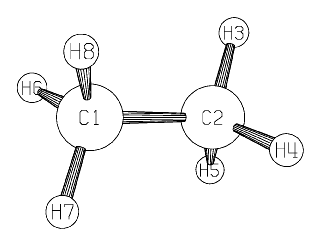
\includegraphics{picc2h6}
\end{center}

\begin{verbatim}
SYMMETRY
ETHANE, D3D                NA NB NC

C
C    1.53 1                 1
H    1.10 1  110 1          2  1
H    1.10 0  110 0  120 0   2  1  3
H    1.10 0  110 0  240 0   2  1  3
H    1.10 0  110 0   60 0   1  2  3
H    1.10 0  110 0  180 0   1  2  3
H    1.10 0  110 0  300 0   1  2  3
0    0.00 0    0 0    0 0   0  0  0
3,    1,    4,    5,     6,     7,     8,
3,    2,    4,    5,     6,     7,     8,
\end{verbatim}
\caption{\label{c2h6} Ethane, showing use of \comp{SYMMETRY}}
\end{figure}

\begin{table}
\caption{\label{xsym} Cartesian Coordinate Symmetry Functions}
\begin{makeimage}
\end{makeimage}
\begin{enumerate}
\item[1] X coordinate is set equal to   the reference X coordinate
\item[2] Y coordinate is set equal to   the reference Y coordinate
\item[3] Z coordinate is set equal to   the reference Z coordinate
\item[4] X coordinate is set equal to $-$ the reference X coordinate
\item[5] Y coordinate is set equal to $-$ the reference Y coordinate
\item[6] Z coordinate is set equal to $-$ the reference Z coordinate
\item[7] X coordinate is set equal to   the reference Y coordinate
\item[8] Y coordinate is set equal to   the reference Z coordinate
\item[9] Z coordinate is set equal to   the reference X coordinate
\item[10] X coordinate is set equal to $-$ the reference Y coordinate
\item[11] Y coordinate is set equal to $-$ the reference Z coordinate
\item[12] Z coordinate is set equal to $-$ the reference X coordinate
\item[13] X coordinate is set equal to   the reference Z coordinate
\item[14] Y coordinate is set equal to   the reference X coordinate
\item[15] Z coordinate is set equal to   the reference Y coordinate
\item[16] X coordinate is set equal to $-$ the reference Z coordinate
\item[17] Y coordinate is set equal to $-$ the reference X coordinate
\item[18] Z coordinate is set equal to $-$ the reference Y coordinate
\end{enumerate}
\end{table}

Usually a lower heat of formation can be obtained when  \comp{SYMMETRY}  is
specified.   To  see  why,  consider  the  geometry  of  benzene.   If no
assumptions are made regarding  the  geometry,  then  all  the  C--C bond
lengths  will  be very slightly different, and the angles will be almost, but
not quite 120 degrees.  Fixing all angles at 120  degrees,  dihedrals at  180
or 0 degrees, and only optimizing one C--C and one C--H bond-length will
result  in  a  2--D optimization, and exact D$_{6h}$ symmetry. Any deformation
from  this  symmetry  must  involve  error,  so  by imposing symmetry some
error is removed.


The layout of the symmetry data is:
\\
\comp{$<$defining atom$> <$symmetry relation$> <$defined atom$> <$defined atom$>$,\ldots}
\\
where the numerical codes for \comp{$ <$symmetry relation$>$} are given
in the tables of symmetry functions, (Tables~\ref{isym} and \ref{xsym}).

For function 19 in internal coordinates, the format of the symmetry data is
\\
\comp{$<$defining atom$> $ 19 $<$multiplying factor$> <$defined atom$> <$defined atom$>$,\ldots}
\\

For example,  ethane,  with  three  independent  internal coordinate
variables,  can  be defined as shown in Figure~\ref{c2h6}. Here atom 3,  a
hydrogen,  is  used  to  define  the  bond  lengths (symmetry  relation  1)
of  atoms  4,5,6,7 and 8 with the atoms they are specified to bond with in the
NA column of the data file; similarly,  its angle  (symmetry  relation  2)  is
used to define the bond-angle of atoms 4,5,6,7 and 8 with the two atoms
specified in the NA and  NB  columns  of the  data  file.   The other angles
are point-group symmetry defined as a multiple of 60 degrees.

Spaces, tabs or commas can be used to separate data.  Note that only three
parameters  are  marked to be optimized.  The symmetry data can be the last
line of the data file unless more data follows, in which case  a blank line
must be inserted after the symmetry data.


Internal coordinate symmetry function  19  (see Table~\ref{isym})  is
intended  for  use  in   polymers,  in  which   the translation  vector  may be
a multiple of some bond-length.  1,2,3 and 14 are most commonly used.
Abbreviation:  \comp{SYM}.


Methane, specified using Cartesian coordinates, can be described with
one unknown, the C--H bond length, as shown in Figure~\ref{xch4}.

\begin{figure}
\begin{makeimage}
\end{makeimage}
\begin{verbatim}
XYZ  SYMMETRY
Methane, Td

C   0.0000000 0    0.0000000 0    0.0000000 0
H   0.6375302 1    0.6375302 0    0.6375302 0
H   0.6375302 0   -0.6375302 0   -0.6375302 0
H  -0.6375302 0    0.6375302 0   -0.6375302 0
H  -0.6375302 0   -0.6375302 0    0.6375302 0

   2  1    3
   2  4    4   5
   2  9    2   5
   2 12    3   4
   2 14    2   4
   2 17    3   5
\end{verbatim}
\caption{\label{xch4} Example of Cartesian \comp{SYMMETRY} functions}
\end{figure}

\subsection*{\comp{T-PRIORITY} (O)}
\index{T--PRIORITY}
\index{DRC}
In  a  DRC  calculation,  results  will  be  printed  whenever   the
calculated time changes by 0.1 femtoseconds.  Abbreviation, T-PRIO.
See Section~\ref{t_irc} for more details.


\subsection*{\comp{T-PRIORITY=$n.nn$} (O)}
In  a  DRC  calculation,  results  will  be  printed  whenever   the
calculated time changes by $n.nn$ femtoseconds.


\subsection*{\comp{T=$n$[M,H,D]} (W)}
\index{T=$n$}
This is a facility to allow the program to shut down in  an  orderly
manner on computers with execution time cpu  limits.

The total cpu  time allowed for the current  job  is  limited  to \index{Cpu
time!specification} $nn.nn$  seconds;  by default this is one hour, i.e., 3600
seconds.  If the next cycle of the calculation cannot be completed without
running a  risk of  exceeding the assigned time the calculation will write a
restart file and then stop.  The safety margin is 100 percent; that is, to do
another cycle, enough time to do at least two full cycles must remain.

If several systems are run in one job, then the time allowed for {\em all} the
jobs is one hour, unless \comp{T=$n.nn$} is used.  If \comp{T=$n.nn$} is used,
then the allowed time {\em for the remainder of the job} is $n.nn$ seconds.
This means that if the allowed time for each system is to be an hour, then the
keyword \comp{T=1h} must be specified in each system.


Alternative specifications of the time are  \comp{T=$nn.nn$M},  which  defines
the  time in minutes, \comp{T=$nn.nn$H}, in hours, and \comp{T=$nn.nn$D}, in
days, for very long jobs.

\subsection*{\comp{THERMO} (O)}
\index{THERMO|ff}
\index{Heat capacity}
\index{Partition function}
\index{Internal!energy}
\index{Entropy}

The  thermodynamic  quantities,  internal  energy,  heat   capacity, partition
function,  and  entropy  can  be  calculated~\cite{thermo}   for translation,
rotation and vibrational degrees of freedom for a single temperature,  or a
range  of temperatures.  Special situations such as linear systems and
transition states are  accommodated.   The  approximations  used  in  the
THERMO  calculation  are  invalid  below  100K, and checking of the lower bound
of the temperature range is done to prevent  temperatures  of  less than 100K
being used. See Section~\ref{tsuneo} for more detail.

Another limitation, for which no checking is  done,  is  that  there should
be  no  internal  rotations.   If  any  exist,  they  will not be recognized as
such, and the calculated quantities will be too  low  as  a result.

If \comp{THERMO} is specified on its own, then the default  values  of  the
temperature  range  are  assumed.   This  starts at 200K and increases in steps
of 10 degrees to 400K.  Three  options  exist  for  overriding  the default
temperature range.  These are:

\subsection*{\comp{THERMO($nnn$) or THERMO=($nnn$) } (O)}
The thermodynamic quantities for a 200 degree range of temperatures,
starting at $nnn$K (integer) and with an interval of 10 degrees
are to be calculated.

\subsection*{\comp{THERMO($nnn$,$mmm$) or THERMO=($nnn$,$mmm$) } (O)}
The thermodynamic quantities for the temperature range limited by  a
lower bound of $nnn$ Kelvin and an upper bound of $mmm$ Kelvin (both integer
numbers), the step size
being calculated  in  order  to  give  approximately  20  points,  and  a
reasonable  value  for  the step.  The size of the step in Kelvin degrees
will be 1, 2, or 5, or a power of 10 times these numbers.

\subsection*{\comp{THERMO($nnn$,$mmm$,$lll$) or THERMO=($nnn$,$mmm$,$lll$) } (O)}
Same as for \comp{THERMO($nnn$,$mmm$)}, (three integer numbers) only now the
user can explicitly define
the step size.  The step size, $lll$, cannot be less than 1K.

\subsection*{\comp{THRESH=$n.nn$} (W)}
\index{THRESH}
In \comp{TIDY} the LMOs are tidied up:  this involves deleting atoms that have
very low intensity in an LMO, and removing the unused space that is generated
as a result.  The intensity, $\rho$,  of an atom in a LMO is given by:
\begin{equation}
\rho_A=\sum_{\lambda\epsilon A}\psi_{\lambda}^2
\end{equation}
The criterion for `very low intensity' has a default of
10$^{-10}$, and can be reset by \comp{THRESH=$n.nn$}.  See also \comp{RELTHR}.

\subsection*{\comp{TIDY} (O)} \index{TIDY}
Some of the working in \hyperref[pageref]{subroutine \comp{TIDY}}{ (See
p.~}{)}{tidy} is printed when \comp{TIDY} is specified.

\subsection*{\comp{TIMES} (O)}
\index{TIMES}
The times for various stages of the calculation are printed when \comp{TIMES}
is specified.  This is very useful in finding out what is using a lot of
time.  A second use is to find out precisely where in a run a failure occurred.

\subsection*{\comp{TOM} (O)}
\index{TOM}
The \htmlref{MIERTUS-SCROCCO-TOMASI self-consistent reaction field
model}{mst} for solvation is used when \comp{TOM} is specified.

\begin{latexonly}
For more detail on this technique, see page~\pageref{mst}.
\end{latexonly}

When \comp{TOM} is specified, an additional keyword (\comp{H2O},
\comp{CHCL3}, or \comp{CCL4}) is necessary or \htmlref{extra
data must be supplied}{mstdata} at the end of the input file.

\begin{latexonly}
A description of this data is given on page~\pageref{mstdata}.
\end{latexonly}

\subsection*{\comp{TRANS} (C)} \index{TRANS}
    The imaginary frequency due to the reaction vector in  a
    transition state calculation must not be included in the
   thermochemical calculation.  The number of genuine vibrations
   considered can be:
    $3N-5$ for a linear ground state system, $3N-6$ for a
    non-linear ground state system, or $3N-6$ for a linear
    transition-state complex, $3N-7$ for a non-linear
    transition-state complex.

        This keyword must be used in conjunction with \comp{THERMO} if
a transition state is being calculated.



\subsection*{\comp{TRANS=$n$ } (C)}
        The facility exists  to  allow  the  THERMO  calculation  to  handle
   systems  with  internal  rotations.   \comp{TRANS=$n$}  will  remove  the $n$ lowest
   vibrations.  Note that \comp{TRANS=1} is equivalent to \comp{TRANS} on  its  own.   For
   xylene, for example, \comp{TRANS=2} would be suitable.


\subsection*{\comp{TRIPLET} (C)}
\index{TRIPLET|ff}
        The triplet state is defined.  In order to define this type of calculation
other keywords {\em must} also be used.  For a `simple' triplet calculation,
use \comp{C.I.=2}.  Results from such calculations can be compared with
ground state calculations.
If the triplet state consists of two half-filled degenerate M.O.s,
such as molecular oxygen,
then \comp{OPEN(2,2)} should be used.

From experience,  \comp{OPEN(2,2)} and \comp{TRIPLET} run faster
than \comp{C.I.=2} and \comp{TRIPLET}.

 If the system has an  odd  number  of
   electrons,  an error message will be printed.

See also \comp{SINGLET}, \comp{DOUBLET}, \comp{QUARTET}, \comp{QUINTET},
\comp{SEXTET}, \comp{SEPTET}, \comp{OCTET},  and \comp{NONET}.

UHF interpretation:

        The number of alpha electrons exceeds that of the beta electrons  by
   2.   If  \comp{TRIPLET}  is  not  specified,  then the numbers of alpha and beta
   electrons are set equal.  This  does  not  necessarily  correspond  to  a
   singlet.

RHF interpretation:

        \comp{TRIPLET} cannot be used unless other keywords are present. If
\comp{C.I.=2} is used, then a single state corresponding to:
$$
\frac{1}{\sqrt{2}}(\psi_{homo}^{\alpha}.\psi_{lumo}^{\beta}+\psi_{homo}^{\beta}.\psi_{lumo}^{\alpha})
$$
is calculated.
   See keywords \comp{C.I.=$n$} and \comp{OPEN($n_1$,$n_2$)}.
\index{Configuration interaction}

 When the configuration interaction calculation is done, all microstates having
a component of spin,  M$_S$, equal to   1 are selected.  These microstates are then
used in the construction of states.  Because of the way in which the microstates
were chosen, only states of spin equal to or greater than   1 can be constructed.
From this set, only a triplet state can be selected, all other states will be ignored.
If \comp{ROOT=$n$} is present, then the $n$'th triplet state will be selected,
otherwise the first triplet state will be  chosen.

\subsection*{\comp{TS} (C)}
\index{TS|ff}
\index{Gradient!minimization!using TS}
        Within the Eigenvector  Following  routine~\cite{ef-ts},  the
   option  exists  to
   optimize   a   transition  state.   To  do  this,  use  \comp{TS}.   Preliminary
   indications are that the TS method is much faster and more reliable  than
   either SIGMA or NLLSQ.

        \comp{TS} appears to work well with Cartesian coordinates.

        In the event that TS does not converge on a  stationary  point,  try
   adding \comp{RECALC=5} to the keyword line.



\subsection*{\comp{UHF} (C)}
\index{UHF|ff}
\index{Unrestricted Hartree-Fock}
        The unrestricted Hartree-Fock Hamiltonian is to be used.

\subsection*{\comp{UNSAFE} (W)}
\index{UNSAFE}\label{unsafe}
If MOPAC has been compiled so that the special SCF convergers can be used,
then the memory demand will be higher than if they are not allowed.
These convergers are not needed for well-behaved systems, and therefore
more memory is needed than is used.
To reduce the memory demand for a run, add \comp{UNSAFE} to the keyword line.
A side effect of this command is that some systems will fail to generate an SCF,
and the run may be wasted as a result. Do not use \comp{UNSAFE} unless there
is a need to conserve memory resources.

\subsection*{\comp{VDW($text$)} (W)}
\index{VDW}
\index{Atoms!making fully ionic}
\index{Elements!making fully ionic}
\index{VDW}\label{key_vdw}
\index{Van der Waals!radii, changing}

The Van der Waals radii of atoms can be set or changed by use of \comp{VDW}.
The format of the command is:

\comp{VDW(:$<$chemical symbol$_1>$=$n.nn$:$<$chemical symbol$_2>$=$n.nn$:$<$chemical symbol$_3>$=$n.nn$:\ldots)}

For example, \comp{VDW(:Cl=2.33:Br=2.50)} would override the default values
of the van der Waals radii of chlorine and bromine (1.65 and 1.80, respectively).
Note that all chemical symbols (including the first one) must be preceded
by a colon (:).

This keyword is used in setting the VDW radii in the COSMO solvation method.

The VDW radii are also used in determining connectivity in  the generation of
the Lewis structure.  Thus, to make sure that a magnesium  atom is  fully
ionic, the keyword \mbox{\comp{VDW(:Mg=--1.0)}} could be used.  Note that a
large negative VDW  radius ensures that no atoms are within the VDW radius.

\subsection*{\comp{VECTORS} (O)}
\index{VECTORS}

\comp{MOPAC:}

\index{Eigenvectors!printing}
        The eigenvectors are to be printed.  In UHF calculations both  alpha
   and  beta  eigenvectors  are printed; if \comp{ALLVEC} is specified,
   in all cases the full set, occupied
   and virtual, are output.  By default, the nine highest occupied and the
seven lowest unoccupied levels
are printed.  The eigenvectors are normalized to unity:  that
   is, the  sum of the squares of the coefficients is exactly one.  If \comp{DEBUG}
   is specified, then the eigenvectors  on  {\em every}  iteration  of  every  SCF
   calculation  will  be printed.  This is useful in a learning context, but
   would normally be undesirable.

\comp{MOZYME:}

\index{Eigenvectors!printing}
The molecular orbitals are printed if \comp{VECTORS} is present.  The type
of M.O.s printed depends on the presence of another keyword, \comp{EIGEN}.

        If \comp{EIGEN} is {\em not} present, then
the final set of occupied localized molecular orbitals is to be printed.


If \comp{EIGEN} is  present, then the conventional M.O.s or eigenvectors
are printed.
By default, only the M.O.s near the HOMO-LUMO gap are printed.  In order
to print all the M.O.s, use the keywords \comp{VECTORS}, \comp{EIGEN}, and
\comp{ALLVECS}.
(O)



\subsection*{\comp{VELOCITY} (C)}
\index{VELOCITY}
\index{DRC!use of VELOCITY}
The user can supply the initial  velocity  vector  to  start  a  DRC
calculation.  For obvious reasons, the input  geometry  should  be  in
Cartesian coordinates.  If internal coordinates must be used, add \comp{GEO-OK}.

        Put the velocity vector after the geometry as three data  per  line,
   representing  the  $x$, $y$, and $z$ components of velocity for each atom.  The
   units of velocity are centimeters per second.

        If \comp{KINETIC=$n.n$} is also specified, the velocity vector will be scaled
   to  equal  the  velocity corresponding to $n.n$ kcal/mol.  This allows the
   user to define the direction of the velocity  vector;  the  magnitude  is
   given by \comp{KINETIC=$n.n$}.

\subsection*{\comp{WILLIAMS} (C)}
\index{WILLIAMS}
        Within the ESP calculation, the Connolly  surface  is  used  as  the
   default.   If  the  surface  generation  procedure  of Donald Williams is
   wanted, the keyword \comp{WILLIAMS} should be used.



\subsection*{\comp{X-PRIORITY} (O)}
\index{X--PRIORITY}
\index{DRC!use of X-PRIORITY}
        In  a  DRC  calculation,  results  will  be  printed  whenever   the
   calculated  geometry  changes  by 0.05~\AA.  The geometry change is
   defined as the linear sum of the translation vectors of  motion  for  all
   atoms in the system.  Abbreviation, \comp{X-PRIO}.
See Section~\ref{t_irc} for more details.



\subsection*{\comp{X-PRIORITY=$n.nn$} (O)}
        In  a  DRC  calculation,  results  will  be  printed  whenever   the
   calculated geometry changes by $n.nn$~\AA.

\subsection*{\comp{XENO} (O)} \index{XENO}\label{xeno} By default,
MOZYME only recognizes the standard twenty amino-acid residues, but
some proteins contain residues which have extra molecular fragments
attached.  In order to allow these unusual species to be recognized,
the keyword \comp{XENO} is provided.

\comp{XENO}, from the Greek $\xi\acute{\epsilon}\nu o\varsigma$, xenos,
for `stranger', defines the unusual species in terms of the extra atoms
which are added to the normal residue.  The format of \comp{XENO} is:

\comp{XENO=($n_C$,$n_N$,$n_O$,$n_S$,$name$[;$n_C$,$n_N$,$n_O$,$n_S$,$name$][;$n_C$,$n_N$,$n_O$,$n_S$,$name$]\ldots)}

Up to four fragments can be defined.  To specify a fragment, the number
of extra carbon, nitrogen, oxygen, and sulfur atoms in the fragment is
used.  A $name$ should be selected which describes the fragment.

As an example, consider the extra fragment in bacteriorhodopsin, on
Lys216:

$\chem  -COCHRNH- ;  R = \chem{CH_2CH_2CH_2CH_2N\!\!=\!\!CHCH\!\!=\!\!CMeCH\!\!=\!\!CHCH\!\!=\!\!CMeCH\!\!=\!\!CHC_9H_{15}}$

Not counting hydrogens, the empirical formula for a lysine fragment is
$\chem C_6N_2O$ (Table~\ref{aacids}
\begin{latexonly}
, p.~\pageref{aacids}
\end{latexonly}).  For residue 216, the empirical
formula is $\chem C_{26}N_2O$, so the extra fragment, the Schiff base,
accounts for $\chem C_{20}$.  Therefore, the number of extra atoms is,
in the order C, N, O, S, `20,0,0,0'.  To specify the retinal fragment,
the keyword would be \comp{XENO=(20,0,0,0,RETINAL)}.

Only the number of extra atoms for the elements C, N, O, and S need be
specified, because these are the elements used in identifying the
residues.  Thus, a phosphorylated serine, of formula:
$\chem{-COCHRNH- ; R = CH_2\! -\! (H_2PO_4)}$
would be specified by the keyword
\comp{XENO(0,0,3,0,PO4)}.

In the output, all the atoms of the residue are labeled with the three
letter abbreviation of the amino-acid.  Ideally, the atoms of the extra
fragment would be labeled differently, but it is not easy to
algorithmically `recognize' the fragment.  Instead, the unusual residue
is indicated in the residue sequence  by an asterisk ($*$), and a
one-line description given immediately before the sequence is printed.

If \comp{XENO} is {\em not} used, the calculation will still work, but
the label for the modified fragment will be \comp{UNK}, instead of the
more descriptive label which would result from using \comp{XENO}.

\subsection*{\comp{XYZ} (W)} \index{XYZ|ff}
   Regardless of the coordinate system used in defining the geometry,
   if \comp{XYZ} is present, then all atoms will be converted to
Cartesian coordinates, and the calculation will be run entirely in
Cartesian coordinates.

        When a large ring system is being optimized,  the closure  is sometimes
   difficult, in which case \comp{XYZ} will normally work.

\subsection{Keywords that go together}
 Normally only a subset of keywords are used in any  given  piece  of
 research.  Keywords which are related to each other in this way are:

\begin{enumerate}
\item In getting an SCF:  \comp{SHIFT}, \comp{PULAY}, \comp{ITRY},
\comp{CAMP}, \comp{SCFCRT}, \comp{1SCF}, \comp{PL}.
\item In MECI work:  \comp{SINGLET}, \comp{DOUBLET}, etc.,
\comp{OPEN($n$,$m$)}, \comp{C.I.=($n$,$m$)}, \comp{CIS}, \comp{CISD},
\comp{PECI}, \comp{CISDT}, \comp{LARGE}, \comp{MECI}, \comp{MS=$n$},
\comp{VECTORS}, \comp{ESR}, \comp{ROOT=$n$}, \comp{MICROS}. See
Section~\ref{meci} for more details.
\item In excited states: \comp{UHF} with (\comp{TRIPLET}, \comp{QUARTET},
etc.), \comp{C.I.=$n$}, \comp{C.I.=($n$,$m$)}. See Section~\ref{meci} for more
details.
\item In geometry optimization:
\begin{enumerate}
\item  Using BFGS: \comp{GNORM=$n.n$}, \comp{XYZ}, \comp{PRECISE}.
\item Using EF: \comp{GNORM=$n.n$}, \comp{XYZ}, \comp{PRECISE}, \comp{NOUPD},
\comp{RSCAL}, \comp{NONR}, \comp{GNMIN}, \comp{CYCLES}, \comp{RECALC},
\comp{IUPD}, \comp{MODE}, \comp{DDMIN}, \comp{DDMAX}, \comp{DMAX}, \comp{HESS},
\comp{RMIN}, \comp{RMAX}, \comp{OMIN}.

\item Using NLLSQ: \comp{GNORM=$n.n$}, \comp{XYZ}, \comp{PRECISE}
\item Using SIGMA: \comp{GNORM=$n.n$}, \comp{XYZ}, \comp{PRECISE}
\end{enumerate}
\item In COSMO calculations: \comp{RSOLV}, \comp{DISEX}, \comp{NSPA},
\comp{VDW}, \comp{EPS}.
\item In Gaussian work: \comp{AIGIN}, \comp{AIGOUT}, \comp{AIDER}.
\item In SADDLE: \comp{BAR=$n.n$}
\item In DRC or IRC: see Section~\ref{t_irc} for more details.
\end{enumerate}

See also Sections \ref{chadef}, \ref{t_irc} and Chapter \ref{criteria} for
other keywords that are usually associated together.
